\chapter{Spin \& angular momentum addition}
In preparation, instead of a scalar wave function $\Psi(\vec{r})$ we consider a vector-valued wave function with three components, $\vec{\Psi}(\vec{r})=[\Psi_x,\Psi_y,\Psi_z](\vec{r})$ and study its behavior under rotations. This consideration will naturally lead us to the concept of spin $\vec{S}$ as the internal degree of freedom of the particle. We will also see that the intrinsic spin $\vec{S}$ and the orbital angular momentum $\vec{L}$ add up to the total angular momentum $\vec{J}=\vec{L}+\vec{S}$ and we have to understand how to handle such an angular momentum addition. In the following, we first discuss some general properties of the spin before we come to the angular momentum addition in Chapter 11.3, where we turn to the Clebsch-Gordan technique. Towards the end of the chapter, we will consider some physical examples, the muon spin rotation, the basics of NMR spectroscopy, today particularly relevant in the context of processing quantum information, the Zeeman effect and spin-orbit coupling (in the hydrogen atom).

\section{Vector-valued wave function $\vec{\Psi}(\vec{r})$}
We start with the usual scalar wave function $\Psi(\vec{r})$ and consider its behavior with a rotation of $\vec{w}$,
%公式 1
\begin{equation}
    \left(U_{\vec{\omega}} \Psi\right)(\vec{r})=\Psi_{\vec{\omega}}(\vec{r})=\Psi\left(\mathbf{R}_{\vec{\omega}}^{-1} \vec{r}\right)
    \end{equation}
For small $\vec{w}$ we approximate the rotation via
%公式 2
$$\mathbf{R}_{\vec{\omega}} \vec{r}=\vec{r}+\vec{\omega} \wedge \vec{r}$$
\begin{equation}
\mathbf{R}_{\vec{\omega}}=\left(\begin{array}{ccc}{1} & {-\omega_{z}} & {\omega_{y}} \\ {\omega_{z}} & {1} & {-\omega_{x}} \\ {-\omega_{y}} & {\omega_{x}} & {1}\end{array}\right)
\end{equation}
and we find the rotated wave function
% 3
\begin{equation}
\begin{aligned} U_{\vec{\omega}} \Psi(\vec{r}) &=\Psi(\vec{r}-\vec{\omega} \wedge \vec{r}) \\ & \cong \Psi(\vec{r})-\vec{\omega} \wedge \vec{r} \cdot \vec{\nabla} \Psi(\vec{r}) \\ &=\Psi(\vec{r})-\frac{i}{\hbar} \vec{\omega} \wedge \vec{r} \cdot \vec{p} \Psi(\vec{r}) \\ &=\Psi(\vec{r})-\frac{i}{\hbar} \vec{\omega} \cdot \vec{L} \Psi(\vec{r}) \end{aligned}
\end{equation}
with $\vec{L}=\vec{r}\wedge\vec{p}$ as usual. Next we consider the vector valued wave function $\vec{\Psi}(\vec{r})$ and also rotate it around $\vec{w}$,
%公式 4
\begin{equation}
    U_{\vec{\omega}} \vec{\Psi}(\vec{r})=\vec{\Psi}_{\vec{\omega}}(\vec{r})=\mathbf{R}_{\vec{\omega}} \vec{\Psi}\left(\mathbf{R}_{-\vec{\omega}} \vec{r}\right)
    \end{equation}
Inserting (11.2) gives
%公式 5
\begin{equation}
\begin{aligned} U_{\vec{\omega}} \vec{\Psi}(\vec{r}) &=\mathbf{R}_{\vec{\omega}} \vec{\Psi}\left(\mathbf{R}_{-\vec{\omega}} \vec{r}\right) \\ & \cong \vec{\Psi}(\vec{r}-\vec{\omega} \wedge \vec{r})+\vec{\omega} \wedge \vec{\Psi}(\vec{r}) \\ &=\vec{\Psi}(\vec{r})-\frac{i}{\hbar} \vec{\omega} \cdot \vec{L} \vec{\Psi}(\vec{r})+\vec{\omega} \wedge \vec{\Psi}(\vec{r}) \\ &=\left[11-\frac{i}{\hbar} \vec{\omega} \cdot(\vec{L} 11+\vec{S})\right] \vec{\Psi}(\vec{r}) \end{aligned}
\end{equation}
with $\vec{\omega} \wedge \vec{\Psi}=-(i / \hbar) \vec{\omega} \cdot \vec{S} \vec{\Psi}$, where the vector operator $\vec{S}$ is given by the following three matrices,
%公式 6
\begin{equation}
\begin{aligned} S_{x} &=i \hbar\left(\begin{array}{ccc}{0} & {0} & {0} \\ {0} & {0} & {-1} \\ {0} & {1} & {0}\end{array}\right) \\ S_{y} &=i \hbar\left(\begin{array}{ccc}{0} & {1} & {0}\end{array}\right) \\ S_{y} &=i \hbar\left(\begin{array}{ccc}{0} & {0} & {1} \\ {0} & {0} & {0} \\ {-1} & {0} & {0}\end{array}\right) \\ S_{z} &=i \hbar\left(\begin{array}{ccc}{0} & {-1} & {0} \\ {1} & {0} & {0} \\ {0} & {0} & {0}\end{array}\right) \end{aligned}
\end{equation}
or
%公式 7
\begin{equation}
    \left(S_{i}\right)_{j k}=-i \hbar \varepsilon_{i j k}
    \end{equation}
The infinitesimal generators (11.7) are unit-equivalent to the $l = 1$ generators in Table 4.1. We identify $\vec{J}=\vec{L}+\vec{S}$ with the total angular momentum of the particle. $\vec{L}$ deals with the $\vec{r}$-dependence without mixing the vector components and we identify $\vec{L}$ with the orbital angular momentum. $\vec{S}$ acts on the components of $\vec{\Psi}$, i.e. $\vec{S}$ rotates the `structure of the particle' without influencing the coordinate $\vec{r}$ and we identify $\vec{S}$ with an `inner' angular momentum of the particle, the particle spin, here $s = 1$. \par This structure can be generalized: instead of a vector-valued wave function, we can generally use a spinor with 2, 3, 4,. , , Consider k components — the matrices (11.6) are then replaced by the infinitesimal generators for $s = (k - 1) / 2$. For $k = 2$ we get the spin-1/2 characteristic of many elementary particles. The above consideration somewhat demystifies the concept of spin; spin is nothing more than an internal structure that forces us to consider a spinor-valued wave function, whereby the $(k-)$ spinor behaves under rotation of space according to the corresponding representation in $k = 2s + 1$ dimensional Hilbert space.
\section{General properties of the spin}
Many elementary particles such as electrons, protons, neutrons, muons or neutrinos have an 'inner' angular momentum. If one measures these angular momentum along an axis, one finds the values ​​$\hbar/2$ and $-\hbar/2$; it is said that the particle has the spin 1/2. The spin shows all the characteristics of an angular momentum and we therefore introduce the spin operator $\vec{S}=(S_x, S_y, S_z)$,
%公式 8
\begin{equation}
    \left[S_{i}, S_{j}\right]=i \hbar \varepsilon_{i j k} S_{k}
    \end{equation}
Since only two values ​​are measured, we introduced the abstract Hilbert space $\mathcal{H}_{1/2}$, with dim $\mathcal{H}_{1/2} = 2$. We construct a base in $\mathcal{H}_{1/2}$ by using the two commutating operators $\vec{n}\cdot\vec{S}$ and $S^2$ (with a direction vector $\vec{n}$) Diagonalize at the same time, see Chapter 4. For example, let $\vec{n}=\vec{e}_z$, then is
%公式 9
\begin{equation}
    |s, m\rangle=\left|\frac{1}{2}, \pm \frac{1}{2}\right\rangle
    \end{equation}
a base in $\mathcal{H}_{1/2}$. Since $s = 1/2$ is fixed, we omit this quantum number. In general we then write for the basis, which is defined by $\vec{n} \cdot \vec{S}, S^{2}$ as
%公式 
\begin{equation}
    |\vec{n} \uparrow\rangle, \quad|\vec{n} \downarrow\rangle
    \end{equation}
With
%公式
\begin{equation}
\begin{aligned} S^{2}|\vec{n} \uparrow\rangle &=\frac{3 \hbar^{2}}{4}|\vec{n} \uparrow\rangle, & S^{2}|\vec{n} \downarrow\rangle &=\frac{3 \hbar^{2}}{4}|\vec{n} \downarrow\rangle \\ \vec{n} \cdot \vec{S}|\vec{n} \uparrow\rangle &=\frac{\hbar}{2}|\vec{n} \uparrow\rangle, & \vec{n} \cdot \vec{S}|\vec{n} \downarrow\rangle &=-\frac{\hbar}{2}|\vec{n} \downarrow\rangle \end{aligned}\nonumber
\end{equation}
For the basis defined by $\vec{n}=\vec{e}_z$ we write briefly $|\uparrow\rangle$ and $ |\downarrow\rangle$. A general spin state $| \Psi\rangle$ can be written as $(\alpha,\varphi\in\mathbb{R})$
\begin{equation}
    |\Psi\rangle=\frac{1}{\sqrt{1+\alpha^{2}}}\left[|\uparrow\rangle+\alpha e^{i \varphi}|\downarrow\rangle\right]=\langle\uparrow | \Psi\rangle|\uparrow\rangle+\langle\downarrow | \Psi\rangle|\downarrow\rangle
    \end{equation}
%公式 11
and represent as a vector on the Bloch sphere, cf. Fig.11.1. Often writes
%图 1
\begin{figure}[ht]
    \begin{minipage}{0.5\textwidth}
        \centering
        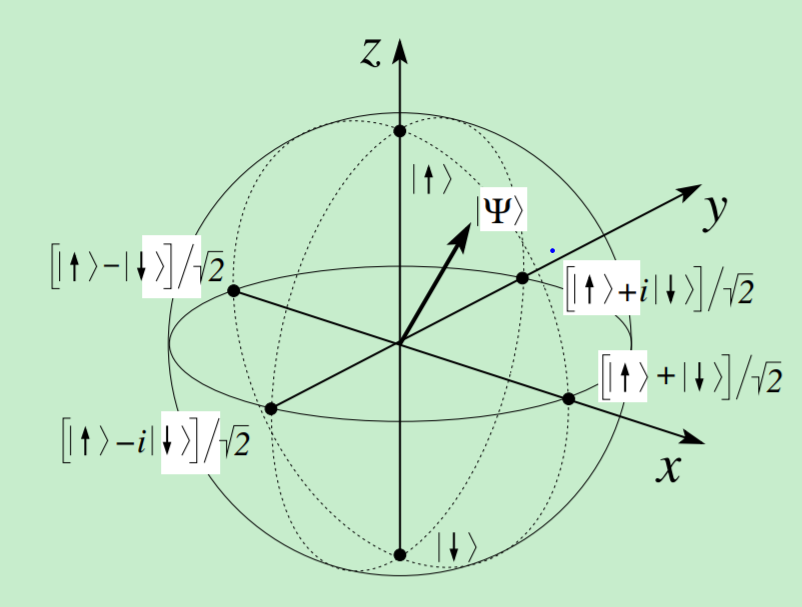
\includegraphics[scale=0.8]{11_1.PNG}
    \end{minipage}
    \begin{minipage}{0.5\textwidth}
        \captionsetup{font={Large}}
        \caption{Each spin state $| \Psi\rangle$ corresponds to a vector of the Bloch sphere.}
    \end{minipage}
\end{figure}
one also the spinor
% 12
\begin{equation}
\Psi=\left(\begin{array}{c}{\alpha} \\ {\beta}\end{array}\right), \quad|\uparrow\rangle=\left(\begin{array}{c}{1} \\ {0}\end{array}\right), \quad|\downarrow\rangle=\left(\begin{array}{c}{0} \\ {1}\end{array}\right)
\end{equation}
The representation of the operators $S_x,S_y,S_z$ in this basis is given by
%公式 13
\begin{equation}
    \vec{S}=\frac{\hbar}{2} \vec{\sigma}
    \end{equation}
with the Pauli Spin matrices (see page 144, table 4.1)
%公式 14
\begin{equation}
\sigma_{x}=\left(\begin{array}{cc}{0} & {1} \\ {1} & {0}\end{array}\right), \quad \sigma_{y}=\left(\begin{array}{cc}{0} & {-i} \\ {i} & {0}\end{array}\right), \quad \sigma_{z}=\left(\begin{array}{cc}{1} & {0} \\ {0} & {-1}\end{array}\right)
\end{equation}
The Pauli matrices have some useful properties:
%公式 15
\begin{eqnarray}
\sigma_{i} \sigma_{j}-\sigma_{j} \sigma_{i} &=&2 i \varepsilon_{i j k} \sigma_{k} \\ \sigma_{i} \sigma_{j} &=&i \varepsilon_{i j k} \sigma_{k}, \quad i \neq j \\ \sigma_{i} \sigma_{j}+\sigma_{j} \sigma_{i} &=&2 \delta_{i j} \mathbb{1} \\ \Rightarrow \sigma_{i}^{2}=\mathbb{1}, & &\sigma_{i} \sigma_{j}=-\sigma_{j} \sigma_{i}, \quad i \neq j \nonumber\\ \sigma_{i} \sigma_{j} &=&\delta_{i j}\mathbb{1}+i \varepsilon_{i j k} \sigma_{k} \end{eqnarray}
%公式 16
%公式 17
%公式 18
Proof: (11.15) follows from (11.8) and (11.16) can be found by recalculating. (11.17) follows from (11.16) for $i\neq j$. The relationship $\sigma_i^2=\mathbb{1}$ is again proven by recalculating. (11.18) follows from (11.15) and (11.17)
The following also applies to any $\vec{a}$ and $\vec{b}$:
%公式 19
\begin{equation}
\begin{aligned}(\vec{a} \cdot \vec{\sigma})(\vec{b} \cdot \vec{\sigma}) &=a_{i} b_{j} \sigma_{i} \sigma_{j}=a_{i} b_{j}\left(\delta_{i j}+i \varepsilon_{i j k} \sigma_{k}\right) \\ &=(\vec{a} \cdot \vec{b})+i(\vec{a} \wedge \vec{b}) \cdot \vec{\sigma} \end{aligned}
\end{equation}
$\vec{S}$ defines due to (11.8) rotations in $\mathcal{H}_{1/2}$. A general rotation around $\vec{w}$ is done by the operator
\begin{equation}
    U_{\vec{\omega}}=\exp [-i \vec{S} \cdot \vec{\omega} / \hbar]
    \end{equation}
%公式 20
described. For example, $\vec{n}$ results from a rotation by $\vec{w}$ from the unit vector $\vec{m}$ as sketched in Figure 11.2, then is
%图 2
\begin{figure}[ht]
    \begin{minipage}{0.5\textwidth}
        \centering
        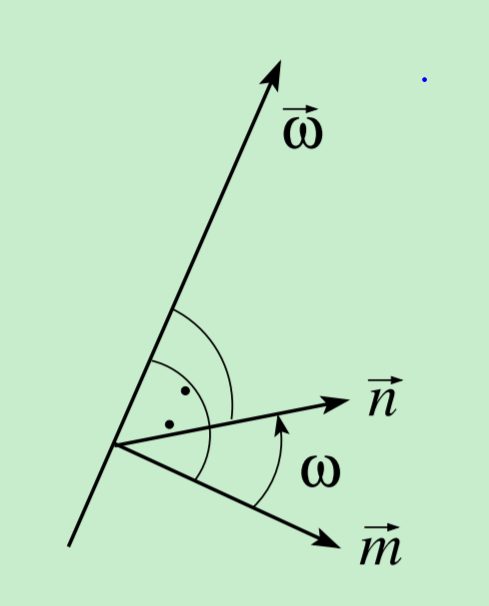
\includegraphics[scale=1]{11_2.PNG}
    \end{minipage}
    \begin{minipage}{0.5\textwidth}
        \captionsetup{font={Large}}
        \caption{Rotation from $\vec{m}$ to $\vec{n}$ around $\vec{w}$: axis $\hat{w}$, angle $w$.}
    \end{minipage}
\end{figure}
%公式 21
\begin{equation}
    \vec{S} \cdot \vec{n}=e^{-i \vec{S} \cdot \vec{\omega} / \hbar} \vec{S} \cdot \vec{m} e^{i \vec{S} \cdot \vec{\omega} / \hbar}
    \end{equation}
and transferred to the states $|\vec{m}\uparrow\rangle$ and $|\vec{m}\downarrow\rangle$
%公式 22
\begin{equation}
    |\vec{n} \uparrow\rangle= e^{-i \vec{S} \cdot \vec{\omega} / \hbar}|\vec{m} \uparrow\rangle, \quad|\vec{n} \downarrow\rangle= e^{-i \vec{S} \cdot \vec{\omega} / \hbar}|\vec{m} \downarrow\rangle
    \end{equation}
\textbf{Proof (11.21):} For small $\vec{w},\vec{n}=\vec{m}+\vec{\omega} \wedge \vec{m}$ and
%公式 23
\begin{equation}
\begin{aligned} \vec{S} \cdot \vec{n} & \approx(11-(i / \hbar) \vec{S} \cdot \vec{\omega}) \vec{S} \cdot \vec{m}(11+(i / \hbar) \vec{S} \cdot \vec{\omega}) \\ &=\vec{S} \cdot \vec{m}+\frac{i}{\hbar}[\vec{S} \cdot \vec{m}, \vec{S} \cdot \vec{\omega}] \\ &=(\vec{S} \cdot \vec{m})+\frac{i}{4 \hbar} \underbrace{[(\vec{\sigma} \cdot \vec{m})(\vec{\sigma} \cdot \vec{\omega})-(\vec{\sigma} \cdot \vec{\omega})(\vec{\sigma} \cdot \vec{m})]}_{2 i \vec{\sigma} \cdot(\vec{m} \wedge \vec{\omega})} \\ &=\vec{S} \cdot \vec{m}-\vec{S} \cdot(\vec{m} \wedge \vec{\omega})=\vec{S} \cdot(\vec{m}+\vec{\omega} \wedge \vec{m}) \end{aligned}
\end{equation}
Proof (11.22): We apply (11.21) to $e^{-i \vec{S} \cdot \vec{\omega} / \hbar}|\vec{m} \uparrow\rangle$,
%公式 
\begin{equation}
\begin{aligned} \vec{S} \cdot \vec{n}\left(e^{-i \vec{S} \cdot \vec{\omega} / \hbar}|\vec{m} \uparrow\rangle\right) &=e^{-i \vec{S} \cdot \vec{\omega} / \hbar} \underbrace{\vec{S} \cdot \vec{m}|\vec{m} \uparrow\rangle}_{\frac{\hbar}{2}|\vec{m} \uparrow\rangle} \\ &=\frac{\hbar}{2}\left(e^{-i \vec{S} \cdot \vec{\omega} / \hbar}|\vec{m} \uparrow\rangle\right)=\frac{\hbar}{2}|\vec{n} \uparrow\rangle \end{aligned}
\end{equation}
and likewise for $|\vec{n}\downarrow\rangle$.\par
The rotation $\exp [-i \vec{S} \cdot \vec{\omega} / \hbar]$ can be found in the base $|\uparrow\rangle,|\downarrow\rangle$ just write as
%^公式
\begin{align} e^{-i \vec{\sigma} \cdot \vec{\omega} / 2} &=\sum_{n=0}^{\infty} \frac{(-i \vec{\sigma} \cdot \vec{\omega} / 2)^{n}}{n !} \\ &=\sum_{n=2 k} \frac{(-i \omega / 2)^{n}}{n !} \mathbb{1}+\sum_{n=2 k+1} \frac{(-i \omega / 2)^{n}}{n !} \hat{\omega} \cdot \vec{\sigma} \\
&=\mathbb{1} \cos \frac{\omega}{2}-i \hat{\omega} \cdot \vec{\sigma} \sin \frac{\omega}{2}
\end{align}
%公式 27
In the step from (11.25) to (11.26) we used the relationship $(\vec{w}\cdot\vec{\sigma})^2=w^2\mathbb{1}$. With this we get for the $|\vec{n}\uparrow\rangle$ state represented in the $\vec{z}$ basis
%公式 28
\begin{equation}
|\vec{n} \uparrow\rangle= e^{-i \vec{S} \cdot \vec{\omega} / \hbar}\left(\begin{array}{c}{1} \\ {0}\end{array}\right)=\left(\begin{array}{c}{\cos \frac{\omega}{2}-i \hat{\omega}_{z} \sin \frac{\omega}{2}} \\ {\left(-i \hat{\omega}_{x}+\hat{\omega}_{y}\right) \sin \frac{\omega}{2}}\end{array}\right)
\end{equation}
where $\vec{w}$ turns straight $\vec{z}$ to $\vec{n}$.\par
\textbf{Note:}
%公式 
\begin{equation}
\begin{aligned}
\left(\begin{array}{c}
    \langle\uparrow | \vec{n} \uparrow\rangle\\
    \langle\downarrow | \vec{n} \uparrow\rangle
\end{array}\right) &=\left(\begin{array}{c}{\langle\uparrow | \exp [-i \vec{\sigma} \cdot \vec{\omega} / 2] i\rangle\langle i | \uparrow\rangle} \\ {\langle\downarrow | \exp [-i \vec{\sigma} \cdot \vec{\omega} / 2] j\rangle\langle j | \uparrow\rangle}\end{array}\right) \\ &=\left(\mathbb{1} \cos \left(\frac{\omega}{2}\right)-i \hat{\omega} \cdot \vec{\sigma} \sin \frac{\omega}{2}\right)\left(\begin{array}{l}{1} \\ {0}\end{array}\right) 
\end{aligned}
\end{equation}
There is a quantization axis $\vec{n}$ for each spin state $|\Psi\rangle$, so that
\begin{equation}
    (\vec{S} \cdot \vec{n})|\Psi\rangle=\frac{\hbar}{2}|\Psi\rangle
    \end{equation}
%公式 30
\textbf{Proof:} via (11.28) each  $\left(\begin{array}{c}\alpha\\\beta
\end{array}\right)$ defines an axis of rotation $\vec{w}$, which is transformed into $\left(\begin{array}{c}\alpha\\\beta
\end{array}\right)$ in $\left(\begin{array}{c}1\\0
\end{array}\right)$ basis.
The rotation by $2\pi$ gives
%公式 31
\begin{equation}
    \exp [-i \vec{\sigma} 2 \pi \vec{e} / 2]=\mathbb{1}] \cos \pi-i \vec{e} \cdot \vec{\sigma} \;\sin \pi=-\mathbb{1}
    \end{equation}
With that, the rotations
%公式 32
\begin{equation}
    U_{\vec{\omega}} \quad \text { and } \quad U_{(\omega+2 \pi) \hat{\omega}}=U_{\vec{\omega}} \underbrace{U_{2 \pi \hat{\omega}}}_{-\mathbb{1}}=-U_{\vec{\omega}}
    \end{equation}
in Hilbert space $\mathcal{H}_{1/2}$ represents the same rotation in $\mathbb{R}^3$: the representation is two-valued,
%公式 33
\begin{equation}
    R_{\vec{\omega}} \in S O(3) \quad \longrightarrow \quad \pm U_{\vec{\omega}} \in S U(2)
    \end{equation}
Since only expected values ​​that are bilinear in $|\Psi\rangle$ can be measured, there are no problems due to the ambiguity, because the wave function and especially its phase cannot be measured directly, only relative phases are relevant: $\langle\Phi, \Psi\rangle=\langle\widetilde{\Phi}, \widetilde{\Psi}\rangle \operatorname{with} \widetilde{\Psi}, \widetilde{\Phi}=U_{2 \pi \hat{\omega}} \Psi, U_{2 \pi \hat{\omega}} \Phi$. The differences in $SO (3)$ versus $SU (2)$ are shown schematically in Figure 11.3.\par
\textbf{Note:}
%公式 34
\begin{equation}
\begin{aligned} \operatorname{det} U_{\vec{\omega}} &=\operatorname{det} e^{-i \vec{\sigma} \cdot \vec{\omega} / 2} \\ &=e^{\operatorname{Sp}(-i \vec{\sigma} \cdot \vec{\omega}) / 2}=e^{0}=1 \end{aligned}
\end{equation}
because Sp$\vec{\sigma}$= 0. With $\vec{\sigma}$ hermitsch, $U_{\vec{w}}$ is unitary and the associated group is $SU (2)$.\par
%图 3
\begin{figure}[ht]
        \centering
        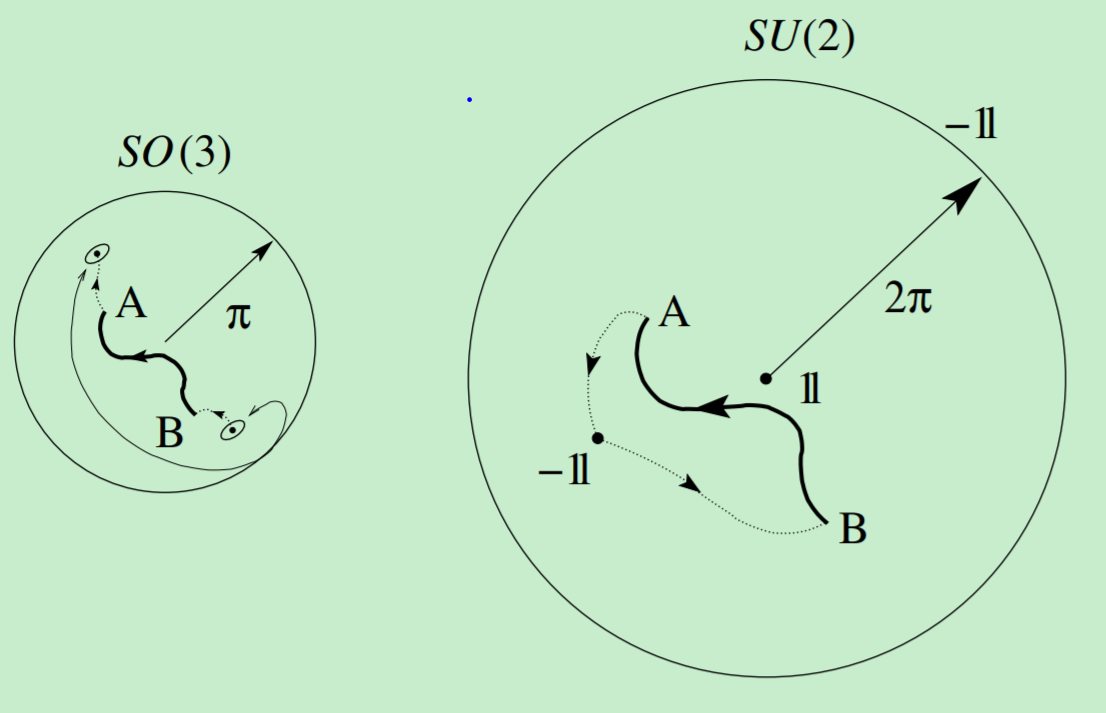
\includegraphics[scale=1]{11_3.PNG}
        \captionsetup{font={Large}}
        \caption{$SO (3)$ versus $SU (2)$: The turning group $SO (3)$ is connected in two ways. Opposing points on the surface (rotation by $\pi$) are to be identified. The path AB closed via the surface cannot be contracted. The group $SU (2)$ is simply connected, $SO (3) = SU (2)$ mod $Z_2, SU (2)$ is the overlay group of $SO (3)$ (with $Z2$ the group with 2 elements, here $Z2 = \{\mathbb{1} , −\mathbb{1}\})$. The surface (rotation by $2\pi$) can be identified with the group element $-\mathbb{1}$. The path AB closed over the surface can be contracted.}
\end{figure}
\section{Angular momentum addition}
We set $\hbar=1$. The problem can be easily illustrated using the example of the addition of two spin 1/2 angular momentum. Let $\vec{S}_1$ and $\vec{S}_2$ be the spins two particles, $[\vec{S}_1,\vec{S}_2] = 0$. The Hilbert space $H$ for describing the two spins is the product space $\mathcal{H}_{1/2}\otimes\mathcal{H}_{1/2}$ and the choice of a direction $\hat{e}_z$ defines one Basis $|i, j\rangle=|i\rangle \otimes|j\rangle$ with $i, j \in\{\uparrow, \downarrow\}$ fixed. The product space is 4-dimensional and we write for the base
%公式 35
\begin{equation}
    |\uparrow, \uparrow\rangle, \quad|\uparrow, \downarrow\rangle, \quad|\downarrow, \uparrow\rangle, \quad|\downarrow, \downarrow\rangle
    \end{equation}
The total spin $\vec{S}=\vec{S}_{1}+\vec{S}_{2}$ of the system is again an angular momentum, because
%公式 36
\begin{equation}
\begin{aligned}\left[S_{i}, S_{j}\right] &=\left[S_{1 i}+S_{2 i}, S_{1 j}+S_{2 j}\right] \\ &=\left[S_{1 i}, S_{1 j}\right]+\left[S_{2 i}, S_{2 j}\right] \\ &=i \varepsilon_{i j k} S_{1 k}+i \varepsilon_{i j k} S_{2 k}=i \varepsilon_{i j k} S_k\end{aligned}
\end{equation}
We can therefore find a basis $ | s, m\rangle$, which does not diagonize $\vec{S}_1$ and $\vec{S}_2$ individually but the total spin, i.e., $S^2$ and $S_z$,
%公式 37
\begin{equation}
\begin{aligned} S^{2}|s, m\rangle &= s(s+1)|s, m\rangle \\ S_{z}|s, m\rangle &= m|s, m\rangle \end{aligned}
\end{equation}
\textbf{Diagonalize using simple arguments}\par
We only solve the problem with a few simple considerations. The Hilbert space $H = \mathcal{H}_{1/2}\otimes \mathcal{H}_{1/2}$ falls into irreducible representations of $S^2$ and $S_z$; the corresponding representations have dimensions $2s + 1$ with $s = 0, 1/2, 1, 3/2, 2, \cdots. $ The basis (11.35) includes dim $H$ = 4 = 1 + 3 = 2 + 2. So either $ \mathcal{H}=\mathcal{H}_0 \oplus \mathcal{H}_1$ or $\mathcal{H} = \mathcal{H}_{1/2} \otimes \mathcal{H}_{1/2}$. The latter alternative, $\mathcal{H}_{1/2} \otimes \mathcal{H}_{1/2}$, contains no spins with $m = \pm 1$, but which occur in (11.35), so $ \mathcal{H}=\mathcal{H}_0 \oplus \mathcal{H}_1$. The basis in $\mathcal{H}= \mathcal{H}_{1/2} \otimes \mathcal{H}_{1/2} = \mathcal{H}_0 \oplus \mathcal{H}_1$ which is $S^2$ and $S_z$ diagonalized
%公式 38
\begin{equation}
\left.
\begin{array}{rl}
\text { Singlet } & \left.|0,0\rangle\qquad \right\}\mathcal{H}_0 \\ 
\text { Triplet } & \left.\begin{array}{l}
    |1,-1\rangle \\ 
    |1,0\rangle \\
    |1,1\rangle
    \end{array}\right\}\mathcal{H}_{1}
\end{array}
\right\}
\mathcal{H}
\end{equation}
\textbf{Diagonalize through arithmetic}\par
The same result can be found by a simple calculation. Since we already have a base in $\mathcal{H}$, cf. (11.35), the new basis $| s,m\rangle$, with which $S^2$ and $S_z$ diagonally through this basis must be printable (this goal is systematically achieved with the help of the Clebsch-Gordan coefficients - see Chap. 11.4). We have to find suitable linear combinations of the base vectors (11.35) to diagonize the $S^2$ and $S_z$. We focus on $S_z$ first. It is
%公式 39
\begin{equation}
\begin{aligned} 
S_{z}|\uparrow, \uparrow\rangle &= 1|\uparrow, \uparrow\rangle, & S_{z}|\downarrow, \downarrow\rangle &=- 1|\downarrow, \downarrow\rangle \\ 
S_{z}|\uparrow, \downarrow\rangle &= 0, & S_{z}|\downarrow, \uparrow\rangle &= 0 \end{aligned}
\end{equation}
so $S_z$ is already diagonal with the eigenvalues ​​0 and $\pm 1$. We just have to find combinations that diagonalize $S^2$. If we want to keep the eigenstates of $S_z$, we can only $|\uparrow,\downarrow\rangle$ and $|\downarrow,\uparrow\rangle$ mix. We calculate ($S_{j \pm}=S_{j x} \pm i S_{j y}, j=1,2$)
\begin{equation}
\begin{array}{rcl}
S^2&=&(\vec{S}_1+\vec{S}_2)^2\\
&=&S_{1}^{2}+S_{2}^{2}+2 \vec{S}_{1} \cdot \vec{S}_{2} \\ 
&=&\frac{3}{2}+2 S_{1 z} S_{2 z}+S_{1+} S_{2-}+S_{1-} S_{2+}\end{array}
\end{equation}
%公式 40
Then
%公式 41
\begin{equation}
\begin{aligned} S^{2}|\uparrow, \uparrow\rangle &= 2|\uparrow, \uparrow\rangle= 1(1+1)|\uparrow, \uparrow\rangle \\ S^{2}|\downarrow, \downarrow\rangle &= 2|\downarrow, \downarrow\rangle= 1(1+1)|\downarrow, \downarrow\rangle \end{aligned}
\end{equation}
and $|\uparrow,\uparrow\rangle$,$|\downarrow,\downarrow\rangle$ belong to an $s = 1$ triplet,
%公式 42
\begin{equation}
\left\{\begin{array}{l}{|\uparrow, \uparrow\rangle=|1,1\rangle} \\ {|\downarrow, \downarrow\rangle=|1,-1\rangle}\end{array}\right.
\end{equation}
(Note: $S_{1+} S_{2-}|\uparrow, \uparrow\rangle= S_{1+}|\uparrow\rangle \otimes S_{2-}|\uparrow\rangle= 0 \otimes \sqrt{\cdots}|\downarrow\rangle= 0$.) We get the missing triplet state $| 1, 0\rangle$ with the help of
%公式 
\begin{equation}
    S_{-}|s, m\rangle=\sqrt{s(s+1)-m(m-1)}|s, m-1\rangle
    \end{equation}
from $| 1, 1\rangle$, so
% 44
\begin{equation}
\begin{aligned}|1,0\rangle &=\frac{1}{\sqrt{2}} S_{-}|1,1\rangle \\ &=\frac{1}{\sqrt{2}}\left(S_{1-}+S_{2-}\right)|\uparrow, \uparrow\rangle \\ &=\frac{1}{\sqrt{2}}(\underbrace{\left.\left.S_{1-| \uparrow}\right\rangle \otimes ||1 \uparrow\right\rangle}_{|\downarrow\rangle \otimes|\uparrow\rangle}+\underbrace{\left.|1| \uparrow\rangle \otimes S_{2-| \uparrow}\right)}_{|\uparrow\rangle \otimes|\downarrow\rangle}) \\ &=\frac{1}{\sqrt{2}}(|\downarrow \uparrow\rangle+|\uparrow \downarrow\rangle) \end{aligned}
\end{equation}
The last state must be orthogonal to $| 1, 0\rangle$ and belongs to $S_z = 0$. Furthermore, it must define a one-dimensional representation, so $S = 0$. Together this results
%公式 45
\begin{equation}
    |0,0\rangle=\frac{1}{\sqrt{2}}(|\downarrow \uparrow\rangle-|\uparrow \downarrow\rangle)
    \end{equation}
So we have the following decompositions of the Hilbert space for two spin 1/2 particles:
%
\begin{equation}
\begin{array}{rcl}
\mathcal{H}_{\frac{1}{2}} \otimes \mathcal{H}_{\frac{1}{2}} &=&\mathcal{H}_{0} \oplus \mathcal{H}_{1} \\
\begin{aligned}
    |\uparrow, \uparrow\rangle =|\uparrow\rangle \otimes|\uparrow\rangle \\|\downarrow, \downarrow\rangle =|\downarrow\rangle \otimes|\downarrow\rangle \\|\downarrow, \uparrow\rangle =|\downarrow\rangle \otimes|\uparrow\rangle \\|\uparrow, \uparrow\rangle =|\uparrow\rangle \otimes|\downarrow\rangle
\end{aligned} & & |0,0\rangle\oplus\left\{\begin{array}{l}
    |1,0\rangle \\ |1,0\rangle \\|1,-1\rangle.
\end{array}\right.
\end{array}
\end{equation}
The above determination of the basis $\{|0,0\rangle,|1,1\rangle,|1,0\rangle,|1,-1\rangle\}$ corresponds exactly to the reduction of $S^2, S_z$ in $\mathcal{H}$. We interpret the result in such a way that the spins are either parallel $( s = 1)$ or antiparallel ($s = 0)$, as shown in Figure 11.4.
%图 4
\begin{figure}[ht]
        \centering
        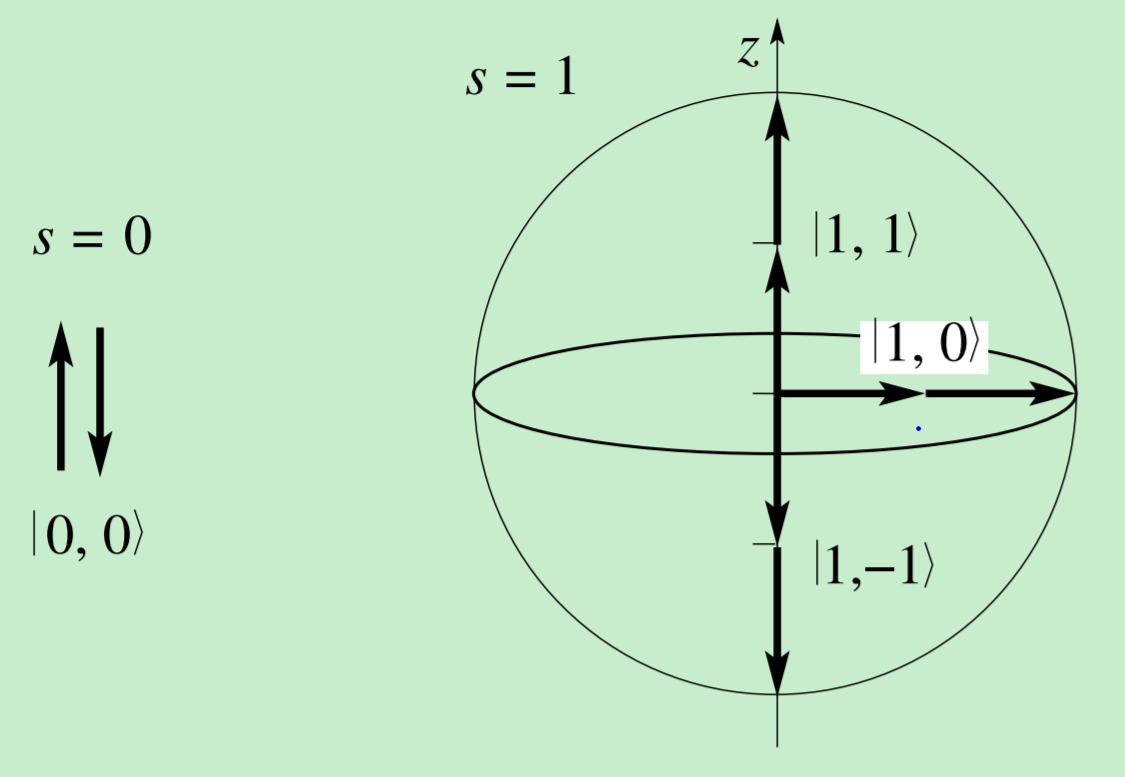
\includegraphics[scale=1]{11_4.PNG}
        \captionsetup{font={Large}}
        \caption{Singlet and triplet eigenstates of the total spin $\vec{S}=\vec{S}_1+\vec{S}_2$ two spin 1/2 particles: left, spin singlet for total spin $s=0,|0,0\rangle=[|\uparrow,\downarrow\rangle-|\downarrow,\uparrow\rangle]/\sqrt{2}$, right, spin triplet states to the total spin $s=1,|1,1\rangle=|\uparrow, \uparrow\rangle,|1,0\rangle=[|\uparrow, \downarrow\rangle+|\downarrow, \uparrow\rangle] / \sqrt{2}$ and $|1,-1\rangle=|\downarrow, \downarrow\rangle$.}
\end{figure}
It is also interesting that $| s, m\rangle$ are eigenstates of $\vec{S}_1,\vec{S}_2$, because
%公式 47
\begin{equation}
    \vec{S}_{1} \cdot \vec{S}_{2}=\frac{1}{2}\left[\left(\vec{S}_{1}+\vec{S}_{2}\right)^{2}-S_{1}^{2}-S_{2}^{2}\right]=\frac{s(s+1)}{2}-\frac{3}{4}
    \end{equation}
Hence for $s = 1$
%公式 48
\begin{equation}
    \vec{S}_{1} \cdot \vec{S}_{2}|1, m\rangle=\left(1-\frac{3}{4}=\frac{1}{4}\right)|1, m\rangle
    \end{equation}
and for ¨ $s = 0$ we get
%公式 49
\begin{equation}
    \vec{S}_{1} \cdot \vec{S}_{2}|0,0\rangle=-\frac{3}{4}|0,0\rangle
    \end{equation}
With that we can use the projectors
%
\begin{equation}
\begin{array}{l}{P_{t}=\frac{3}{4}+\vec{S}_{1} \cdot \vec{S}_{2} \text { to the triplet room, }} \\ {P_{s}=\frac{1}{4}-\vec{S}_{1} \cdot \vec{S}_{2} \text { to the singlet room, }}\end{array}
\end{equation}
define.
\subsection{General case}
We want to add the two angular momentum $\vec{J}_1$ and $\vec{J}_{2},\left[\vec{J}_{1}, \vec{J}_{2}\right]=0$. Starting from the $\left(2 j_{1}+1\right) \times\left(2 j_{2}+1\right)$-dimensional basis $\left|j_{1}, m_{1}\right\rangle \otimes\left|j_{2}, m_{2}\right\rangle \equiv |j_1,j_2,m_1,m_2\rangle$ in the product space $\mathcal{H}=\mathcal{H}_{j_{1}} \otimes \mathcal{H}_{j_{2}}$ we want a new basis $| j_1, j_2 , j, m\rangle$ find, which the operators $J^2$ and $J_z$ to the total angular momentum $\vec{J}=\left(\vec{J}_{1}+\vec{J}_{2}\right)$ simultaneously diagonally. This task is equivalent to reducing the rotation representation in $\mathcal{H}_{j_{1}} \otimes \mathcal{H}_{j_{2}}$, which is available as a product representation. It is
%公式 51
\begin{equation}
\begin{aligned} J_{1}^{2}\left|j_{1}, j_{2}, m_{1}, m_{2}\right\rangle &= j_{1}\left(j_{1}+1\right)\left|j_{1}, j_{2}, m_{1}, m_{2}\right\rangle \\ J_{2}^{2}\left|j_{1}, j_{2}, m_{1}, m_{2}\right\rangle &= j_{2}\left(j_{2}+1\right)\left|j_{1}, j_{2}, m_{1}, m_{2}\right\rangle \\ J_{1 z}\left|j_{1}, j_{2}, m_{1}, m_{2}\right\rangle &= m_{1}\left|j_{1}, j_{2}, m_{1}, m_{2}\right\rangle \\ J_{2 z}\left|j_{1}, j_{2}, m_{1}, m_{2}\right\rangle &= m_{2}\left|j_{1}, j_{2}, m_{1}, m_{2}\right\rangle \end{aligned}
\end{equation}
The sum $\vec{J}=\vec{J}_{1}+\vec{J}_{2}$ is again an angular momentum, so it holds
%公式 52
\begin{equation}
    \left[J_{i}, J_{j}\right]=i \varepsilon_{i j k} J_{k}
    \end{equation}
It is $[J^2, J_z] = 0$, but also $[J^2_i, \vec{J}] = 0$ because $J^2_i$ is a scalar. This is $\left[J_{1}^{2}, J^{2}\right]=0=\left[J_{1}^{2}, J_{z}\right]$ (also for $J_2$) and we can diagonize the operators $J_1^2,J_2^2,J^2$ and $J_z$ at the same time; the corresponding basis $| j_1, j_2, j, m\rangle$ is characterized and fulfilled by the quantum numbers $j_1, j_2, j, m$ (cf. (11.51))
\begin{equation}
\begin{aligned} J_{1}^{2}\left|j_{1}, j_{2}, j, m\right\rangle &= j_{1}\left(j_{1}+1\right)\left|j_{1}, j_{2}, j, m\right\rangle \\ J_{2}^{2}\left|j_{1}, j_{2}, j, m\right\rangle &= j_{2}\left(j_{2}+1\right)\left|j_{1}, j_{2}, j, m\right\rangle \\ J^{2}\left|j_{1}, j_{2}, j, m\right\rangle &= j(j+1)\left|j_{1}, j_{2}, j, m\right\rangle \\ J_{z}\left|j_{1}, j_{2}, j, m\right\rangle &= m\left|j_{1}, j_{2}, j, m\right\rangle \end{aligned}
\end{equation}
%公式 53
We can print out the new base $| j_1, j_2, j, m\rangle$ via Clebsch-Gordan coefficients through the old base,
%公式 54
\begin{equation}
    \left|j_{1}, j_{2}, j, m\right\rangle=\sum_{j_{1}^{\prime}, j_{2}, m_{1}^{\prime}, m_{2}^{\prime}} \underbrace{\left\langle j_{1}^{\prime}, j_{2}^{\prime}, m_{1}^{\prime}, m_{2}^{\prime} | j_{1}, j_{2}, j, m\right\rangle}_{\text {C-G coefficient }}\left|j_{1}^{\prime}, j_{2}^{\prime}, m_{1}^{\prime}, m_{2}^{\prime}\right\rangle
    \end{equation}
Fortunately, many of the C-G coefficients disappear: it is
%公式
\begin{equation}
\begin{aligned}\left\langle j_{1}^{\prime}, j_{2}^{\prime}, m_{1}^{\prime}, m_{2}^{\prime}\left|J_{1}^{2}\right| j_{1}, j_{2}, j, m\right\rangle &= j_{1}^{\prime}\left(j_{1}^{\prime}+1\right)\left\langle j_{1}^{\prime}, j_{2}^{\prime}, m_{1}^{\prime}, m_{2}^{\prime} | j_{1}, j_{2}, j, m\right\rangle \\ &= j_{1}\left(j_{1}+1\right)\left\langle j_{1}^{\prime}, j_{2}^{\prime}, m_{1}^{\prime}, m_{2}^{\prime} | j_{1}, j_{2}, j, m\right\rangle \end{aligned} \nonumber
\end{equation}
so $j_1 = j_1'$ and also $j_2' = j_2$. Furthermore, the matrix elements of $J_z$ result in the condition $m = m_1 + m_2$ (we replace the indices $m_1'$ and $m_2'$ with $m_1$ and $m_2$),
%公式 55
\begin{equation}
\begin{aligned}\left\langle j_{1}, j_{2}, m_{1}, m_{2}\left|J_{z}\right| j_{1}, j_{2}, j, m\right\rangle &=\left(m_{1}+m_{2}\right)\left\langle j_{1}, j_{2}, m_{1}, m_{2} | j_{1}, j_{2}, j, m\right\rangle \\ &= m\left\langle j_{1}, j_{2}, m_{1}, m_{2} | j_{1}, j_{2}, j, m\right\rangle \end{aligned}
\end{equation}
This is how we find the transformation
%公式 56
\begin{equation}
    \left|j_{1}, j_{2}, j, m\right\rangle=\sum_{m_{1}, m_{2} \atop m_{1}+m_{2}=m}\left\langle j_{1}, j_{2}, m_{1}, m_{2} | j_{1}, j_{2}, j, m\right\rangle\left|j_{1}, j_{2}, m_{1}, m_{2}\right\rangle
    \end{equation}
Next we want to list the states, which is trivial in the old basis: Given $j_1$ we have $2j_1 + 1$ states $| j_1, m_1\rangle$, as well as $2j_2 + 1$ states $| j_2, m_2\rangle$, so we get $(2j_1 + 1) × (2j_2 + 1)$ states in the product base $| j_1, j_2, m_1, m_2\rangle$. The new base is more difficult to count down: The diagram shown in Figure 11.5 shows the following:
%公式
\begin{enumerate}
    \item[-] a state with $m=j_{1}+j_{2}=$ maximum, one state with $m=j_{1}+j_{2}=$ maximal,
    \item[-]  two states with $m=j_{1}+j_{2}-1:\left\{\begin{array}{l}{m_{1}=j_{1}, m_{2}=j_{2}-1} \\ {m_{1}=j_{1}-1, m_{2}=j_{2}}\end{array}\right.$
    \item[-] generally this results $j_{1}+j_{2}-m+1$ states with $m \geq\left|j_{1}-j_{2}\right|,$ (the number of options $m_{1}$ and $m_{2}$ on $m=m_{1}+m_{2} \geq\left|j_{1}-j_{2}\right|$ to construct $)$
    \item[-] Further $j_{1}+j_{2}-\left|j_{1}-j_{2}\right|+1=$ const. States with $-\left|j_{1}-j_{2}\right|<m<$
        $\left|j_{1}-j_{2}\right|$
    \item[-] and $j_{1}+j_{2}-|m|+1$ states with $m \leq-|j_{1}-j_{2}|$
\end{enumerate}
What are the possible $j$-states? If we start with the maximum $m_1 + m_2 = m = j_1 + j_2$ there must be $2j + 1$ states for $j = j_1 + j_2$, because from$ | j_1, j_2, j_1 + j_2, j_1 + j_2\rangle$ we can by applying $J_− = J_{1−} + J_{2−}$ in increments of one up to $| j_1, j_2, j_1 + j_2, −j_1 - j_2\rangle$. From the two states with $m = j_1 + j_2−1$ leaves a linear combination (LK) for the $j = j_1 + j_2$ representation, there remains another LK, which $2 (j_1 + j_2−1) + 1$ states other to $j = j_1 + j_2 - 1$ generated, again by iterative application of $J_−$. We can continue this scheme until we get $m= | j_1 − j_2 |$ to reach. As shown in Figure 11.5, no new m states are added. That means we have already created all states $ | j_1, j_2, j, m\rangle$. The total number of states results from simple recounting,
%图 5
\begin{figure}[ht]
        \centering
        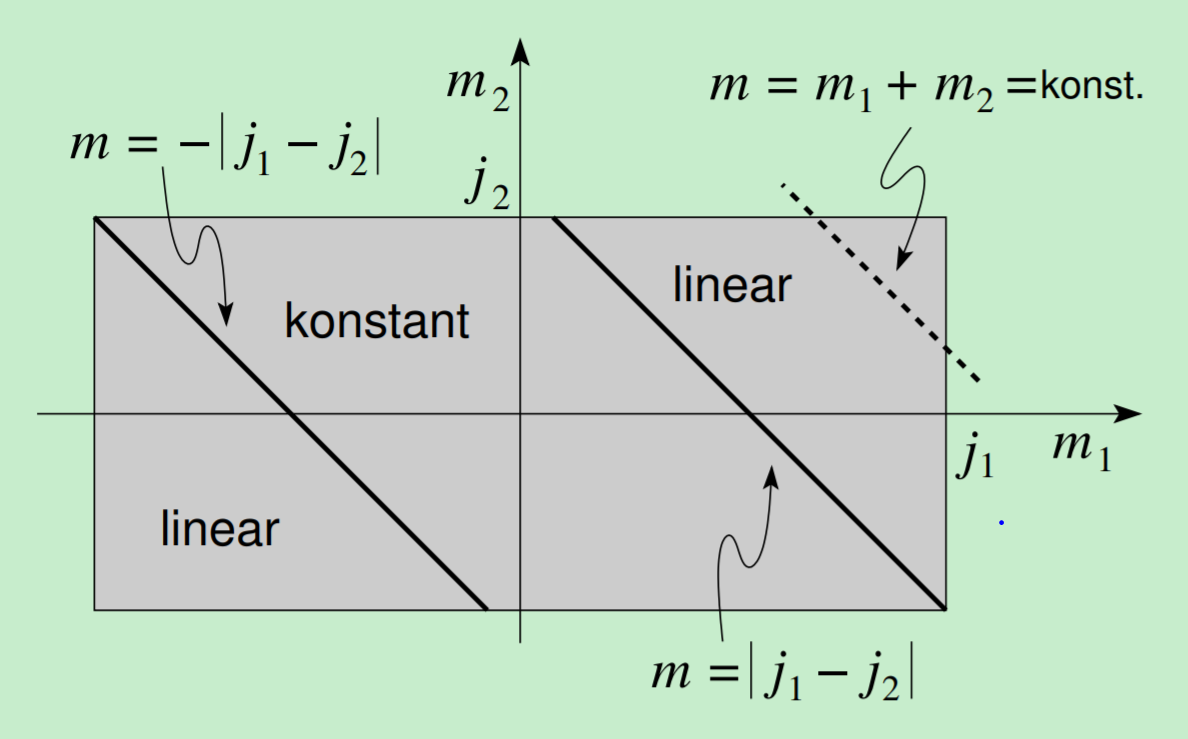
\includegraphics[scale=1]{11_5.PNG}
        \captionsetup{font={Large}}
        \caption{Scheme for counting the eigenstates $| j_1, j_2, j, m\rangle$ to the total angular momentum $j$ of two particles with angular momentum $j_1$ and $j_2$.}
\end{figure}
\begin{equation}
    \sum_{j=\left|j_{1}-j_{2}\right|}^{j_{1}+j_{2}}(2 j+1)=\left(2 j_{1}+1\right)\left(2 j_{2}+1\right)
    \end{equation}
%公式 57
This gives us the decomposition (cf. (11.46))
%公式 58
\begin{equation}
\begin{array}{rlcccc} 
\mathcal{H}_{j_{1}} \otimes \mathcal{H}_{j_{2}}
=& \bigoplus\limits_{j=\left|j_{1}-j_{2}\right|}^{j_{1}+j_{2} |} \mathcal{H}_{j} \\
=& \qquad\mathcal{H}_{\left|j_{1}-j_{2}\right|} & \oplus& \cdots  &\oplus &\mathcal{H}_{j_{1}+j_{2}} \\
&\qquad\qquad\downarrow&&\downarrow\downarrow&&\downarrow\\
& \quad\left|j_{1} j_{2}, j_{1}+j_{2}, j_{1}+j_{2}\right\rangle \\ 
&\qquad\qquad\vdots & && & \vdots \\
&\left|j_{1} j_{2},\right| j_{1}-j_{2}|,-| j_{1}-j_{2}|\rangle & &\cdots&&\quad\left|j_{1 j_{2}, j_{1}}+j_{2},-j_{1}-j_{2}\right\rangle \end{array}
\end{equation}
The product space $\mathcal{H}_{j_{1}} \otimes \mathcal{H}_{j_{2}}$ is represented by the product base $\left|j_{1}, j_{2}, m_{1}, m_{2}\right\rangle=|j_{1}, m_{1}\rangle\otimes|j_2,m_2\rangle$. After we have found the structure of the decomposition of the product space into irreducible `rotation spaces’ $\mathcal{H}_j$, we have to calculate the C-G coefficients so that we can print out the new base using the old and vice versa.

\section{Clebsch-Gordan technology}
To start with: There are Clebsch-Gordan tables, for example A.R. Edmonds, Angular Momentum in Quantum Mechanics (Princeton University Press, New Jersey, 1957) and even web tools for calculating C-G coefficients; Mathematica calculates C-G coefficients via ClebschGordan $[\{j 1, m 1\},\{j 2, m 2\},\{j, m\}]$. Here we discuss how a C-G table is derived. With (11.56) (we suppress the `,' in the vectors),
%公式 
\begin{equation}
    \left|j_{1} j_{2} j m\right\rangle=\sum_{m_{1}, m_{2} \atop m_{1}+m_{2}=m}\left\langle j_{1} j_{2} m_{1} m_{2} | j_{1} j_{2} j m\right\rangle\left|j_{1} j_{2} m_{1} m_{2}\right\rangle
    \end{equation}
the reverse also applies
%公式 60
\begin{equation}
    \left|j_{1} j_{2} m_{1} m_{2}\right\rangle=\sum_{j \atop m=m_{1}+m_{2}}\left\langle j_{1} j_{2} j m | j_{1} j_{2} m_{1} m_{2}\right\rangle\left|j_{1} j_{2} j m\right\rangle
    \end{equation}
The state $\left\langle j_{1} j_{2} m_{1}^{\prime} m_{2}^{\prime}\right|$ applied to (11.60) gives the orthogonality relation
%公式 61
\begin{equation}
\begin{aligned} \sum_{j \atop m=m_{1}+m_{2}}\left\langle j_{1} j_{2} m_{1}^{\prime} m_{2}^{\prime} | j_{1} j_{2} j m\right\rangle\left\langle j_{1} j_{2} j m | j_{1} j_{2} m_{1} m_{2}\right\rangle \\=\delta_{m_{1} m_{1}^{\prime}} \delta_{m_{2} m_{2}^{\prime}} \end{aligned}
\end{equation}
Likewise, $\left\langle j_{1} j_{2} j^{\prime} m^{\prime}\right|$ applied to (11.56) = (11.59) the relationship
%公式 62
\begin{equation}
\begin{aligned} \sum_{m_{1}, m_{2} \atop m=m_{1}+m_{2}}\left\langle j_{1} j_{2} j^{\prime} m^{\prime} | j_{1} j_{2} m_{1} m_{2}\right\rangle\left\langle j_{1} j_{2} m_{1} m_{2} | j_{1} j_{2} j m\right\rangle \\ m=m_{1}+m_{2} \\=& \delta_{j j^{\prime}} \delta_{m m^{\prime}} \end{aligned}
\end{equation}
We can reel all C-G coefficients. We set $j' = j$ and $m' = m$ in (11.62) and normalize the coefficients accordingly
%公式 63
\begin{equation}
    \sum_{m_{1}, m_{2} \atop m=m_{1}+m_{2}}\left\langle j_{1} j_{2} m_{1} m_{2} | j_{1} j_{2} j m\right\rangle^{2}=1
\end{equation}
that means we only have to find the coefficients $\left\langle j_{1} j_{2} m_{1} m_{2} | j_{1} j_{2} j m\right\rangle$ up to a constant factor. To do this, we use the ascent and descent operators and calculate the matrix elements
%公式 64
\begin{equation}
    \left\langle j_{1} j_{2} m_{1} m_{2}\left|J_{\pm}\right| j_{1} j_{2} j m\right\rangle
    \end{equation}
with $J_{\pm}=J_{1 \pm}+J_{2 \pm}$. Applying the operators $J_{\pm}$ to the right gives
%公式 65\
\begin{equation}
\begin{aligned}\left\langle j_{1} j_{2} m_{1} m_{2}\left|J_{\pm}\right| j_{1} j_{2} j m\right\rangle=& \sqrt{j(j+1)-m(m \pm 1)} \\ & \times\left\langle j_{1} j_{2} m_{1} m_{2} | j_{1} j_{2} j m \pm 1\right\rangle \end{aligned}
\end{equation}
while their application left the result
%公式 66
\begin{equation}
\begin{aligned}\left\langle j_{1} j_{2} m_{1} m_{2}\left|J_{\pm}\right| j_{1} j_{2} j m\right\rangle=& \sqrt{j_{1}\left(j_{1}+1\right)-m_{1}\left(m_{1} \mp 1\right)} \\ \times\left\langle j_{1} j_{2} m_{1} \mp 1 m_{2} | j_{1} j_{2} j m\right\rangle & \\+\sqrt{j_{2}\left(j_{2}+1\right)-m_{2}\left(m_{2} \mp 1\right)} & \\ \times\left\langle j_{1} j_{2} m_{1} m_{2} \mp 1 | j_{1} j_{2} j m\right\rangle \end{aligned}
\end{equation}
results. The combination of these relationships results in the triangular recursions (from $J_+$)
%公式 67
\begin{equation}
\begin{aligned} \sqrt{j(j+1)-m(m+1)}\left\langle j_{1 j_{2} m_{1} m_{2}} | j_{1} j_{2} j m+1\right\rangle \\=\sqrt{j_{1}\left(j_{1}+1\right)-m_{1}\left(m_{1}-1\right)}\left\langle j_{1 j 2} m_{1}-1 m_{2} | j_{1 j_{2} j_{2} j m}\right\rangle \\+\sqrt{j_{2}\left(j_{2}+1\right)-m_{2}\left(m_{2}-1\right)}\left\langle j_{1 j_{2} m_{1} m_{2}}-1 | j_{1 j_{2} j m}\right\rangle \end{aligned}
\end{equation}
and (from $J_−$)
\begin{equation}
\begin{aligned} \sqrt{j(j+1)-m(m-1)}\left\langle j_{1} j_{2} m_{1} m_{2} | j_{1} j_{2} j, m-1\right\rangle \\=\sqrt{j_{1}\left(j_{1}+1\right)-m_{1}\left(m_{1}+1\right)}\left\langle j_{1} j_{2} m_{1}+1 m_{2} | j_{1} j_{2} j m\right\rangle \\+\sqrt{j_{2}\left(j_{2}+1\right)-m_{2}\left(m_{2}+1\right)}\left\langle j_{1} j_{2} m_{1} m_{2}+1 | j_{1} j_{2} j m\right\rangle \end{aligned}
\end{equation}
%公式 68
these triangular relations are sketched in Figure 11.6, top right for $J_+$ and bottom left for $J_-$.
%图 6
\begin{figure}[ht]
        \centering
        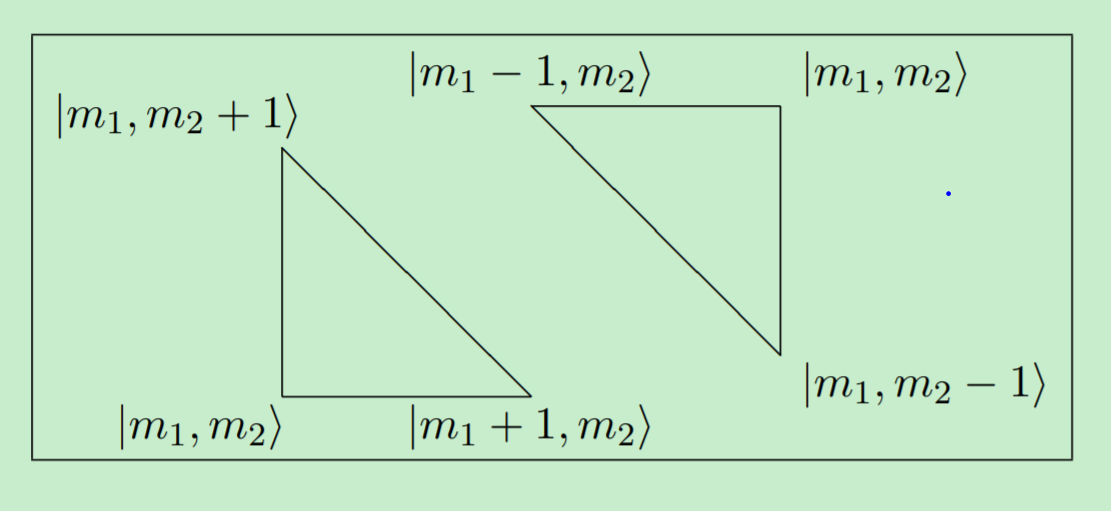
\includegraphics[scale=1]{11_6.PNG}
        \captionsetup{font={Large}}
        \caption{Triangular relationships for $J_+$ (top right) and $J_−$ (bottom left).}
\end{figure}
If two of the coefficients are known, the third follows from the triangular relationships. Our task is to use a fixed but arbitrary $j$ with
%图 7
\begin{figure}[ht]
        \centering
        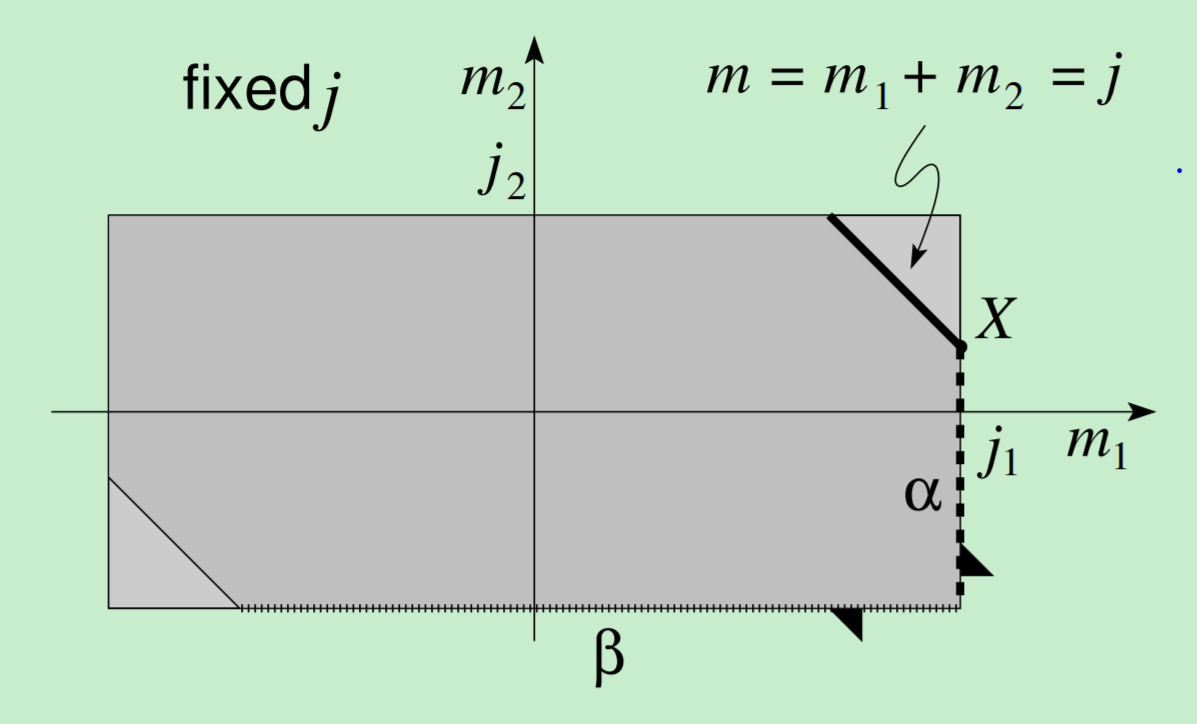
\includegraphics[scale=1]{11_7.PNG}
        \captionsetup{font={Large}}
        \caption{Scheme for calculating the Clebsch-Gordan coefficients: We start at $X$ and use a triangular recursion to find the coefficients along the edge $\alpha$. Using the second triangular recursion gives the edge $\beta$, etc.}
\end{figure}
$\left|j_{1}-j_{2}\right| \leq j \leq j_{1}+j_{2}$ to find the coefficients for all $m_1, m_2$. Consider the diagram sketched in Figure 11.7: we start at point $X$ and choose $\left\langle j_{1} j_{2} j_{1} j-j_{1} | j_{1} j_{2} j j\right\rangle \equiv \nu$ with $\nu\in\mathbb{R}^+$. We follow the edge $\alpha$ using the triangular relation (11.68) (note that $m_2 <(j - j_1))$ and use that for $m_1> j_1$ the coefficient $\left\langle j_{1} j_{2} j_{1}+1 m_{2} | j_{1} j_{2} j j_{1}+1+m_{2}\right\rangle= 0$ vanishes; so we find the recursion
%公式 69
\begin{equation}
\begin{array}{l}{\alpha: \quad \sqrt{j(j+1)-m(m-1)}\left\langle j_{1}, j_{2}, j_{1}, m_{2} | j_{1}, j_{2}, j, m-1\right\rangle} \\ {\quad=\quad \sqrt{j_{2}\left(j_{2}+1\right)-m_{2}\left(m_{2}+1\right)}\left\langle j_{1}, j_{2}, j_{1}, m_{2}+1 | j_{1}, j_{2}, j, m\right\rangle}\end{array}
\end{equation}
We then use (11.67) to generate the values ​​on the edge β and then work iteratively through the matrix. Finally we find ν by normalization (11.63).
The results are particularly simple in the case of the addition of a spin $\vec{S}$ and an angular momentum $\vec{L}$, as used, for example, when determining the total angular momentum of a bound electron. We'll find it
decomposition
%公式 70
\begin{equation}
    \mathcal{H}=\mathcal{H}_{l} \otimes \mathcal{H}_{\frac{1}{2}}=\mathcal{H}_{l+\frac{1}{2}} \oplus \mathcal{H}_{l-\frac{1}{2}}
    \end{equation}
of the Hilbert space product and get the C-G coefficients
$\left\langle l, s, m_{l}, m_{s} | l, s, j, m\right\rangle$ in the form
%公式 71
\begin{equation}
\begin{array}{l}{\text { in } \mathcal{H}_{l+\frac{1}{2}}:\left\langle l, \frac{1}{2}, m \mp \frac{1}{2}, \pm \frac{1}{2} | l, \frac{1}{2}, l+\frac{1}{2}, m\right\rangle=\sqrt{\frac{l \pm m+\frac{1}{2}}{2 l+1}}} \\ {\text { in } \mathcal{H}_{l-\frac{1}{2}}:\left\langle l, \frac{1}{2}, m \mp \frac{1}{2}, \pm \frac{1}{2} | l, \frac{1}{2}, l-\frac{1}{2}, m\right\rangle=\mp \sqrt{\frac{l \mp m+\frac{1}{2}}{2 l+1}}}\end{array}
\end{equation}
Finally, $\vec{S} \cdot \vec{L}$ is diagonal in $|l, s, j, m\rangle$, because
%公式 72
\begin{equation}
    J^{2}=(\vec{L}+\vec{S})^{2}=L^{2}+S^{2}+2 \vec{L} \cdot \vec{S}
    \end{equation}
and with that is
%公式 73
\begin{equation}
    \vec{L} \cdot \vec{S}|l, s, j, m\rangle=\frac{1}{2}\left[j(j+1)-l(l+1)-\frac{3}{4}\right]|l, s, j, m\rangle
    \end{equation}
For $j = l + \frac{1}{2}$, i.e., $\vec{S} \| \vec{L}$, one finds
%公式 74
\begin{equation}
    \vec{L} \cdot \vec{S}\left|l, s, l+\frac{1}{2}, m\right\rangle=\frac{l}{2}\left|l, s, l+\frac{1}{2}, m\right\rangle
    \end{equation}
while for $j = l -\frac{1}{2}$, i.e. $\vec{S}$ antiparallel to $\vec{L}$, the following applies

%公式 75
\begin{equation}
    \vec{L} \cdot \vec{S}\left|l, s, l-\frac{1}{2}, m\right\rangle=-\frac{l+1}{2}\left|l, s, l-\frac{1}{2}, m\right\rangle
    \end{equation}
\subsection{Three angular momentum}
The addition of three angular momentum is done iteratively
%公式 76
\begin{equation}
    \overrightarrow{J_{1}}+\overrightarrow{J_{2}}+\overrightarrow{J_{3}}=(\underbrace{\overrightarrow{J_{1}}+\overrightarrow{J_{2}}}_{\overrightarrow{J_{12}}})+\overrightarrow{J_{3}}=\overrightarrow{J_{1}}+(\underbrace{\overrightarrow{J_{2}}+\overrightarrow{J_{3}}}_{\overrightarrow{J_{23}}})
    \end{equation}
e C-G coefficients are then the sum of products of CG coefficients. The change of basis from the ((12)3) representation to the (1(23)) representation involves the Racah ($W$) coefficients or the Wigner-6j symbols, see special literature, e.g., Edmonds, Angular Momentum in Quantum Mechnanics (Princeton University Press) , As a simple example, examine $\mathcal{H}^{\otimes 3}_{1 / 2} = \mathcal{H}_{1/2} \otimes \mathcal{H}_{1/2} \otimes \mathcal{H}_{1/2} = (\mathcal{H}_0 \oplus \mathcal{H}_1) \otimes \mathcal{H}_{1/2} = 2\mathcal{H}_{1/2} \oplus \mathcal{H}_{3 / 2}$.
\section{ Physical examples}
\subsection{Magnetic moment}
A particle of charge $q (q = −e$ for an electron) and mass $m$, which moves on an orbit with angular momentum $\vec{}$, produces a magnetic moment $\vec{\mu}$ as sketched in Figure 11.8,
%公式 77
\begin{equation}
    \vec{\mu}=\frac{q}{2 m c} \vec{L}
    \end{equation}
%图 8
\begin{figure}[ht]
    \begin{minipage}{0.5\textwidth}
        \centering
        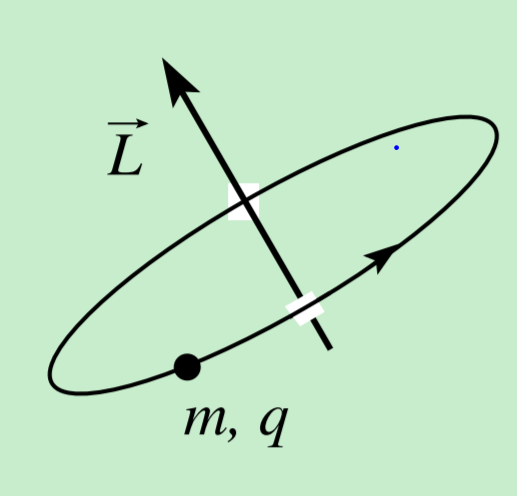
\includegraphics[scale=1]{11_8.PNG}
    \end{minipage}
    \begin{minipage}{0.5\textwidth}
        \captionsetup{font={Large}}
        \caption{Orbital magnetic moment $\vec{\mu}=q\vec{L}/2mc$ of a particle with mass $m$ and charge $q$ in an orbital with angular momentum $\vec{L}$.}
    \end{minipage}
\end{figure}
Similarly, the spin of a particle creates a magnetic moment, even for an uncharged particle (e.g. a neutron, see below). One finds for an electron
%公式 78
\begin{equation}
    \vec{\mu}_{e^{-}}=-g \frac{e}{2 m_{e} c} \vec{S}
    \end{equation}
with the Lande factor $g = 2 + \alpha/\pi$ + terms of higher order in the fine structure constant $\alpha=e^{2} / \hbar c=1 / 137.04$. Note that $\vec{\mu}$ and $\vec{S}$ are antiparallel since $q = −e <0$. For a proton
%公式 79
\begin{equation}
    \vec{\mu}_{p}=g_{p} \frac{e}{2 m_{p} c} \vec{S}, \quad g_{p} \approx 5.59, \quad m_{p}=1.67310^{-27} \mathrm{kg}=1836 \mathrm{m}_{e}
    \end{equation}
and for neutrons
%公式 80
\begin{equation}
    \vec{\mu}_{n}=-g_{n} \frac{e}{2 m_{n} c} \vec{S}, \quad g_{n} \approx 3.83, \quad m_{n}=1.67510^{-27} \mathrm{kg}=1838 \mathrm{m}_{e}
    \end{equation}
If the particle is placed in a magnetic field $\vec{H}$, its energy becomes spin-dependent with the Hamiltonian
%公式 81
\begin{equation}
    H=-\vec{\mu} \cdot \vec{H}
    \end{equation}
Parameters and orders of magnitude: Bohr's magneton defines the energy scale in the problem; it is
%公式 82
\begin{equation}
    \mu_{B}=\frac{e \hbar}{2 m_{e} c}=5.788 \cdot 10^{-9} \mathrm{eV} / \mathrm{Gauss}
    \end{equation}
and with typical laboratory fields in the area $|\vec{H}| \sim 1 \mathrm{T}=10^{4}$ Gauss we get typical energies in the range
%公式 83
\begin{equation}
    \Delta E \approx 10^{-4} \mathrm{eV}=0.1 \mathrm{meV} \approx 1 \mathrm{K} \approx 20 \mathrm{GHz}
    \end{equation}
The saturation field of iron-based materials is in the range of 2 Tesla. Superconducting magnets can generate fields in the range around 20 Tesla, hybrid magnets come up to around 45 Tesla (Tallahassee), pulsed and exploding configurations reach around 100 Tesla.
\subsection{Precession}
If we put a particle with spin into a magnetic field $\vec{H}$, its spin (in general) begins to precision. The dynamic is given by the Hamiltonian (here for an $e^−$)
%公式 84
\begin{equation}
    H(t)=\frac{g \mu_{B}}{\hbar} \vec{S} \cdot \vec{H}(t)
    \end{equation}
In the Heisenberg picture the dynamics are assigned to the operators and we get the evolution equation for the spin (cf. (7.31) (we simplify the notation and write $\vec{S}(t)$ instead of $\vec{S}_H(t)$)

%$公式 85
\begin{equation}
\begin{aligned} i \hbar \partial_{t} S_{i}(t)=\left[S_{i}(t), H(t)\right] &=g \mu_{B}\left[S_{i}(t), S_{j}(t)\right] \mathrm{H}_{j}(t) / \hbar \\ &=i g \mu_{B} \varepsilon_{i j k} S_{k} \mathrm{H}_{j}(t) \end{aligned}
\end{equation}
Here we used that $H_H = H$, which presupposes that $[H (t), H (t')] = 0$. The corresponding condition $\left[\vec{S} \cdot \vec{H}(t), \vec{S} \cdot \vec{H}\left(t^{\prime}\right)\right]=0$ then implies the relation $\left[\vec{H}(t) \wedge \vec{H}\left(t^{\prime}\right)\right] \cdot \vec{\sigma}=0$ and thus it is allowed Magnetic field does not change its direction, $\vec{H}(t)=\vec{H}_{0} f(t)$. The result (11.85) is synonymous with
%公式 86
\begin{equation}
    \partial_{t} \vec{S}(t)=\frac{g \mu_{B}}{\hbar} \vec{S}(t) \wedge \vec{H}(t)=\underbrace{\vec{\mu}(t) \wedge \vec{H}(t)}_{\text {Moment }}
    \end{equation}
i.e. a moment acts on the spin in the magnetic field and the spin begins to precision. In the following example we consider an electron with charge $q = −e$ in the magnetic field $\vec{H}(t)=\left(0,0, \mathrm{H}_{0}\right)$ = const. It is
%图 9
\begin{figure}[ht]
    \begin{minipage}{0.5\textwidth}
        \centering
        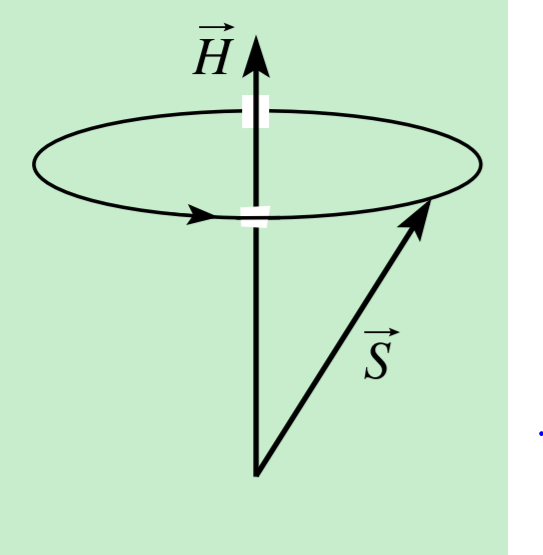
\includegraphics[scale=1]{11_9.PNG}
    \end{minipage}
    \begin{minipage}{0.5\textwidth}
        \captionsetup{font={Large}}
        \caption{Precession of the spin $\vec{S}$ in the magnetic field $\vec{H}$.}
    \end{minipage}
\end{figure}
%公式 87
\begin{equation}
\begin{aligned} \partial_{t} S_{x}(t) &=-\left(g \mu_{B} / \hbar\right) \mathrm{H}_{0} S_{y}(t) \\ \partial_{t} S_{y}(t) &=\left(g \mu_{B} / \hbar\right) \mathrm{H}_{0} S_{x}(t) \\ \partial_{t} S_{z}(t) &=0 \end{aligned}
\end{equation}
with the solution
%公式 88
\begin{equation}
    \begin{array}{ccl}
       \left(\begin{array}{c}{S_{x}(t)} \\ {S_{y}(t)} \\ {S_{z}(t)}\end{array}\right) &=& \left(\begin{array}{ccc}{\cos \omega_{0} t} & {\sin \omega_{0} t} & {0} \\ {-\sin \omega_{0} t} & {\cos \omega_{0} t} & {0} \\ {0} & {0} & {1}\end{array}\right)\left(\begin{array}{c}{S_{x}(0)} \\ {S_{y}(0)} \\ {S_{z}(0)}\end{array}\right)\\
        w_0 &=& -g\mu_BH_0/\hbar
    \end{array}
\end{equation}
With $\left|\omega_{0}\right| / 2 \pi=2.8 \mathrm{MHz} \cdot \mathrm{H}_{0}$ [Gauss] we find typical frequencies in the megahertz to gigahertz range. In the Schrodinger picture, the solution has the form
%公式 89
\begin{equation}
    |\Psi(t)\rangle= e^{-i H t / \hbar}|\Psi(0)\rangle= e^{i \omega_{0} S_{z} t / \hbar}|\Psi(0)\rangle
    \end{equation}
a spin rotating around the $z$-axis with the frequency $w_0$.
\subsection{$\mu$SR-Muon spin rotation}
The muons µ are elementary particles, leptons, with a finite lifetime; they decay directed and emit an electron,
%公式 90
\begin{equation}
    \mu^{-} \rightarrow e^{-}+\nu_{\mu}+\bar{\nu}_{e}
    \end{equation}
with the electron velocity ~ ve preferably directed towards the muon spin S ~ µ, cf. Fig.11.10.

The local magnetic field can be measured by implanting muons in the solid (via muon bombardment), cf. Fig.11.10. The temporal modulation of the count rate in the detector provides the precession frequency ω0, which depends on the local magnetic field strength. The local differences in
%图 10
\begin{figure}[ht]
    \centering
    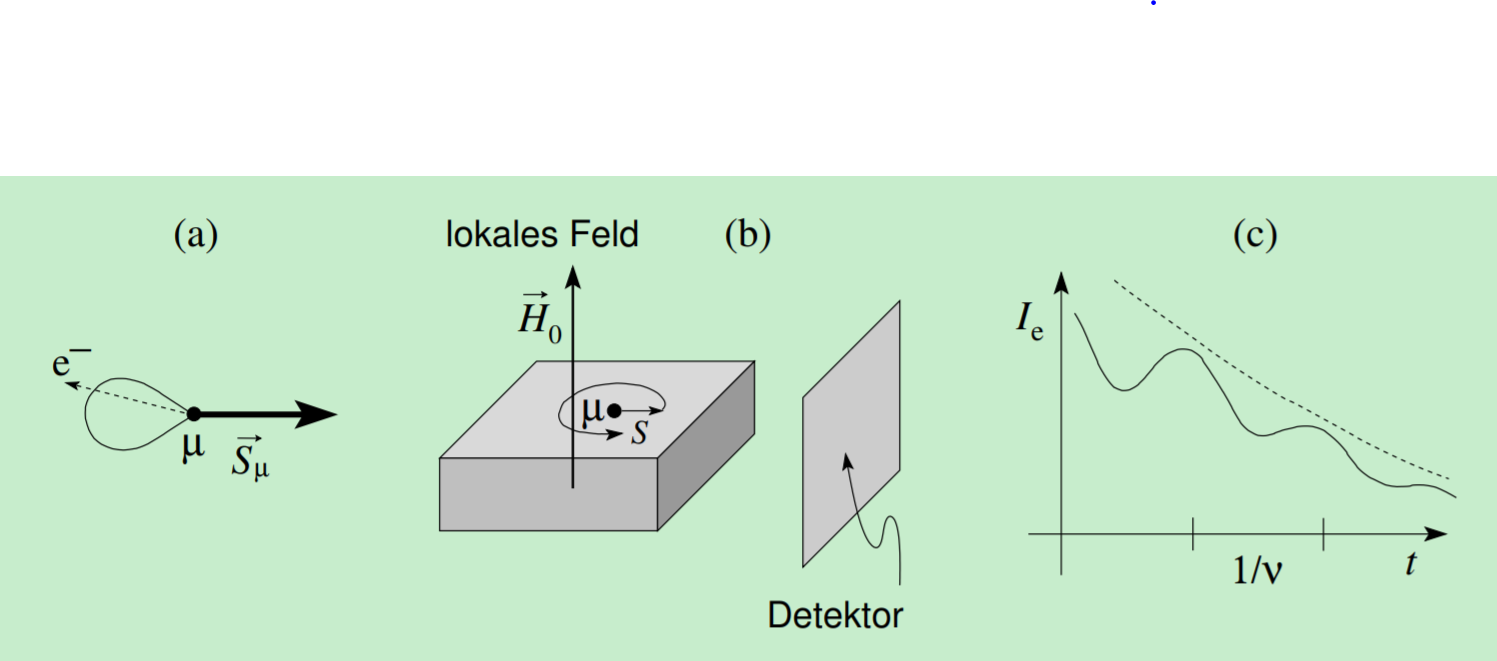
\includegraphics[scale=1]{11_10.PNG}
    \captionsetup{font={Large}}
    \caption{Muon Spin Rotation: $(a)$ A muon decays according to $\mu^-\rightarrow e^-+\nu_{\mu}+\bar{\nu}_e$ and emits the electron preferrably in the direction $-\vec{S}_{\mu}$ against its spin. $(b)$ Muons are caught in the solid; the spin of which occurs according to the local magnetic field $H_0$. That at decay ($\tau_{\mu}=2.2\mu s$) of the electron emitted by the muon is detected and measured. $(c)$ The intensity of the counted electrons $I_e$ oscillates (with frequency $\nu$ according to the strength of the local magnetic field $H_0$. The decay of the intensity (depolarization) is a measure of the variance in the local dimension gnetfeld.}
\end{figure}
Magnetic field result in 'depolarization'. This method can be used to measure spontaneously generated magnetic fields (time invariance-breaking ground states), magnetic ordering phenomena or the penetration depth λ in superconductors (slow muons).

\subsection{NMR - Nuclear Magnetic Resonance - Spin Resonance}
We consider the configuration shown in Figure 11.11 (a). The applied magnetic field consists of a (dominant) dc component $\vec{H}_0$ and an oscillating (ac) component $\vec{H}_1$ perpendicular to it,
% 91
\begin{equation}
    \vec{H}=\vec{H}_{0}+\vec{H}^{\prime}(t)=\left(\mathrm{H}_{1} \cos \omega t, 0, \mathrm{H}_{0}\right)
    \end{equation}
Let $|\Psi(t)\rangle$ be the spin state in the Schrodinger image. $|\Psi(t)\rangle$ is given by the solution of the Schrodinger equation
%公式 92
\begin{equation}
    i \hbar \partial_{t}|\Psi(t)\rangle=-\frac{\mu_{\mathrm{eff}}}{2}\left(\mathrm{H}_{0} \sigma_{z}+\mathrm{H}_{1} \sigma_{x} \cos \omega t\right)|\Psi(t)\rangle
    \end{equation}
%图 11
\begin{figure}[ht]
        \centering
        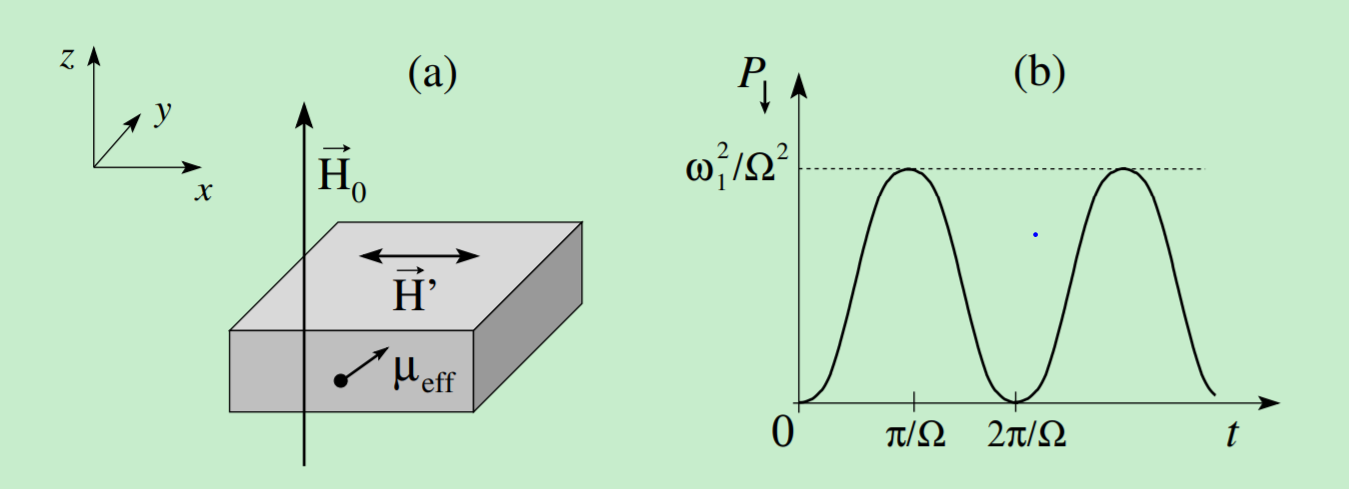
\includegraphics[scale=1]{11_11.PNG}
        \captionsetup{font={Large}}
        \caption{NMR, nuclear magnetic resonance: in a local magnetic field $ H_0 $ with a frequency of $ w_0 = \mu_ {eff} H_0 / \hbar $, the moment ($ \mu _ {\text {eff}} $) (such as a hydrogen atom) is at ( Around $ z $). The transverse AC magnetic field $ H '= H_1 (\operatorname {cos} wt) $ is absorbed by resonance at the frequency $ w = w_0 $, and the magnetic moment is at the frequency $ w_1 = u _ {\text {eff}} H_1 / \hbar $ Rotate (rotate around x). Finding the maximum absorption resonance point can measure the local magnetic field $ H_0 $ and determine the chemical environment by detour. This scheme is also used in quantum computing, where the state of a qubit (= quantum second-order system = effective spin 1/2 system) is controlled by rotation.}
\end{figure}
with the Pauli matrices $\sigma_x$ and $\sigma_z$. With $|\Psi(t)\rangle=\exp \left[i \omega \sigma_{z} t / 2\right]\left|\Psi^{\prime}(t)\right\rangle$ i we get the following equation for the transformed wave function $\left|\Psi^{\prime}(t)\right\rangle$,
\begin{equation}
    i \partial_{t}\left|\Psi^{\prime}(t)\right\rangle=\left[\frac{\omega-\omega_{0}}{2} \sigma_{z}-\omega_{1} \cos \omega t\left(e^{-i \omega \sigma_{z} t / 2} \sigma_{x} e^{i \omega \sigma_{z} t / 2}\right)\right]\left|\Psi^{\prime}(t)\right\rangle
    \end{equation}
%公式 93
with $\omega_{0}=\mu_{\mathrm{eff}} \mathrm{H}_{0} / \hbar$ and $\omega_{1}=\mu_{\mathrm{eff}} \mathrm{H}_{1} / 2 \hbar$. It is
%公式 94
\begin{equation}
\begin{aligned} \sigma_{x}\left(\sigma_{z}\right)^{n} &=\left(-\sigma_{z}\right)^{n} \sigma_{x} \\ \sigma_{x} f\left(\sigma_{z}\right) &=f\left(-\sigma_{z}\right) \sigma_{x} \end{aligned}
\end{equation}
and thus
%公式 95
\begin{equation}
\begin{aligned} e^{-i \omega \sigma_{z} t / 2} \sigma_{x} e^{i \omega \sigma_{z} t / 2} &=\sigma_{x} e^{i \omega \sigma_{z} t} \\ &=\sigma_{x}\left(\cos \omega t+i \sigma_{z} \sin \omega t\right) \end{aligned}
\end{equation}
The equation for $|\Psi^{\prime}(t)$ then has the form (we use the relationships $\cos 2 \omega t=2 \cos ^{2} \omega t-1, \sin 2 \omega t=2 \sin \omega t \cos \omega t$) 
\begin{equation}
    \left.i \partial_{t}\left|\Psi^{\prime}(t)\right\rangle=\left[\frac{\omega-\omega_{0}}{2} \sigma_{z}-\frac{\omega_{1}}{2} \sigma_{x}-\underbrace{\frac{\omega_{1}}{2}\left(\sigma_{x} \cos 2 \omega t+\sigma_{y} \sin 2 \omega t\right)}_{\text {rapidly oscillating } \rightarrow \sim 0}\right] \Psi^{\prime}(t)\right\rangle \nonumber
    \end{equation}
and we get the solution
%公式 96
\begin{equation}
\begin{aligned}\left|\Psi^{\prime}(t)\right\rangle &= e^{-i \Omega \hat{\sigma} t / 2}\left|\Psi^{\prime}(0)\right\rangle \\|\Psi(t)\rangle &= e^{i \omega \sigma_{z} t / 2} e^{-i \Omega \hat{\sigma} t / 2}|\Psi(0)\rangle \end{aligned}
\end{equation}
with $\Omega^{2}=\left(\omega-\omega_{0}\right)^{2}+\omega_{1}^{2},$ and $\hat{\sigma}=\left[\left(\omega-\omega_{0}\right) / \Omega\right] \sigma_{z}-\left(\omega_{1} / \Omega\right) \sigma_{x}$. The `misfit' (detuning) $w-w_0$ between the driver frequency ω and the resonance frequency $w_0$ of the system (here the Zeeman energy) generates a correction for the rotation around the $z$-axis, while the spin is rotated by $x$ with frequency $w_1$ , Let's start with the state $|\Psi(0)\rangle=|\uparrow\rangle$ we get for the probability $P_{\downarrow}(t)=|\langle\downarrow | \Psi(t)\rangle|^{2}$ after time t to measure the reverse spin the result
%公式 97
\begin{equation}
    P_{\downarrow}(t)=\frac{\omega_{1}^{2}}{2 \Omega^{2}}(1-\cos \Omega t)
    \end{equation}
as shown in Figure 11.11 (b). For $\omega \rightarrow \omega_{0}$ is $\Omega \approx \omega_{1}$ and $P_{\downarrow}\left(\pi / \omega_{1}\right) \approx 1$, which means that in the vicinity of the resonance frequency ω0 the probability of turning (or flip) after time $t = \pi / w_1$ is even $\approx 1$ ($\pi$-pulse). The spin extracts $\vec{H}_1$ energy from the rf field (radio-frequency) and turns around. The measurement of the increased absorption at $w = w0$ then indicates the resonance frequency $w_0$ and (with known $\mu_{\text{eff}}$) the value of the local field $\vec{H}_0$. Alternatively, the effective local moment µeff can be found with known field $\vec{H}_0$. This scheme can also be used to manipulate spins - by switching rf fields on and off for precisely defined time intervals, spin states can be changed in a controlled manner. NMR techniques are widely used to find protein configurations in biology. NMR manipulation techniques are used to process quantum information (stored in quantum bits = qubits $|\mathrm{qb}\rangle=[|0\rangle+\alpha \exp (i \varphi)|1\rangle] / \sqrt{1+\alpha^{2}}$, manipulable two-level systems = generalized spin systems).

\textbf{Note:} The result $P_{\downarrow}(t)$ describes transitions of a spin from the state $|\uparrow\rangle$ in the state $|\downarrow\rangle$ under the influence of a microwave field (or transitions of an atom between ground state $| g\rangle$ and excited state $| e\rangle$ under the effect of an optical field). This process is reminiscent of transitions induced by the Fermi Golden Rule. In fact, the topics are closely related but different, they describe Rabi oscillations versus decays of states. In particular, the Rabi oscillations describe the dynamics of a driven 2 level system without the presence of a continuum. A nice example is the atom (excitation) in a cavity (photon) where the excitation oscillates back and forth between the atom and the photon. This suggestion is neither of matter nor of light type in between (a superposition) and is called Polariton (described by the Jaynes-Cummings Model). In contrast, the FGR describes the decay of an excited atom with the emission of a photon, whereby the photon lives in the continuum and flies away. Another FGR process would be the absorption of a photon from the photon field with excitation of the atom. If the emitted photon came back again, for example in a cavity, then it was reabsorbed and re-emitted by the atom and continued periodically, which is nothing more than the Rabi oscillations. Mathematically, the two processes are also related and different: FGR is a result of the 1st order perturbation theory and needs a continuum. Rabi oscillations are described by the exact solution of the Schrodering equation. In the discussion above, the spin takes a photon from the macroscopic, classic microwave field, releases another, picks up another, etc. The macroscopic classic microwave field replaces the photon in the cavity. Also note that FGR gives a probability $\propto t$, but the Rabi oscillations give an oscillation cos$\Omega t (\rightarrow$ summation of the perturbation series). For small $t$, $P_{\downarrow}(t) \propto t^{2}$, which corresponds to the result (9.88) or (9.91), is not the FGR result which describes $P\propto t$ and long times $t$. Furthermore, the FGR is perturbative, so it would never be able to provide a transition probability of order 1 because the disturbance would then be large.

\section{Zeeman effect \& spin-orbit coupling}
If we consider a particle in $\mathbb{R}^3$ with spin 1/2, we describe its state by a product wave function
%公式 98
\begin{equation}
\begin{array}{ccccc}|\Psi\rangle &=\;\left|\Psi_{\mathrm{Bahn}}\right\rangle & \otimes &\left|\chi_{\mathrm{Spin}}\right\rangle \\  & \in & &\in \\ \mathcal{H} &=\;\mathbb{L}_{2}\left(\mathbb{R}^{3}\right) & \otimes &\mathcal{H}_{\frac{1}{2}} \end{array}
\end{equation}
consisting of orbital and spin components. Let us consider the hydrogen atom again as an example. If we switch on a magnetic field $H_z\hat{e}_z$, the Hamiltonian $H_{0}=p^{2} / 2 m-e^{2} / r$ has a magnetic term ($e> 0$)
%公式 99
\begin{equation}
    H_{Z}=\frac{e \mathrm{H}_{z}}{2 m c}\left(L_{z}+g S_{z}\right)
    \end{equation}
to. The second term is known to us from (11.81); the first follows
%公式 100
\begin{equation}
    \vec{p}^{2} \rightarrow(\vec{p}+e \vec{A} / c)^{2}=p^{2}+\frac{e}{c}(\vec{p} \cdot \vec{A}+\vec{A} \cdot \vec{p}) \underbrace{+\frac{e^{2} \vec{A}^{2}}{c^{2}} \vec{A}^{2}}_{\text {Diamagnetismus反磁性}}
    \end{equation}
and with $\vec{A}=-\vec{r} \wedge \overrightarrow{\mathrm{H}} / 2$ we get from it

%公式 101
\begin{equation}
    \frac{\vec{p}^{2}}{2 m} \quad \rightarrow \quad \frac{\vec{p}^{2}}{2 m}+\frac{e}{2 m c} \vec{H} \cdot \vec{L}
    \end{equation}
The second part corresponds exactly to the energy of the magnetic moment $(−e / 2mc)\vec{L}$ in field $\vec{H}$, cf. (11.77).\par
$H_Z$ is not the only term that contains the angular momentum and spin operators. Relativistic effects introduce additional corrections, for example the spin-orbit coupling: The electron moving in the $\vec{\mathcal{E}}$ field of the nucleus emits a magnetic field $\vec{B}=-\vec{v} \wedge \overrightarrow{\mathcal{E}} / c$ whereupon the spin moment coupled. The resulting energy is
%公式 102
\begin{equation}
    -\frac{e}{m c^{2}} \vec{S} \cdot(\vec{v} \wedge \overrightarrow{\mathcal{E}})
    \end{equation}
The Thomas Precession introduces another correction of the same form: this is a relativistic kinematic effect and takes into account that the rest system of the $e^−$ rotates relative to the laboratory system, see Jackson (Electrodynamics), page 541 ff. The correction is just being made to −1/2 times (11.102) and we get the following expression for the spin-orbit coupling (see also Chapter 25, non-relativistic limits of the Dirac equation),
%公式 103
\begin{equation}
\begin{aligned} H_{\mathrm{SO}} &=\frac{-e}{2 m c^{2}} \vec{S} \cdot(\vec{v} \wedge \overrightarrow{\mathcal{E}}) \\ & \downarrow e \overrightarrow{\mathcal{E}}=\vec{\nabla} V=\hat{r} \partial_{r} V(r) \\ &=\frac{1}{2 m c^{2}} \vec{S} \cdot(\vec{r} \wedge \vec{v}) \frac{1}{r} \partial_{r} V \\ &=\frac{1}{2 m^{2} c^{2}} \frac{1}{r} \frac{d V}{d r} \vec{L} \cdot \vec{S} \end{aligned}
\end{equation}
With this we get the Hamiltonian
%公式 104
\begin{equation}
\begin{array}{ccccccccc} 
    H&=&H_{0}&+&\quad H_{\mathrm{Zeman}}&+&\frac{H_{\mathrm{SO}}}{1} \frac{H_{\mathrm{SO}}}{2 \frac{d V}{d r}-\frac{d V}{d r} \vec{L} \cdot \vec{S}} &+& H_R\vspace{1ex}\\ 
    &=&\frac{p^2}{2m}-\frac{e^2}{r}&+&\frac{eH_z}{2mc}(L_z+gS_z)&+&\frac{1}{2m^2c^2}\frac{1}{r}\frac{dV}{dr}\vec{L}\cdot\vec{S}
\end{array}
\end{equation}
and the corrections in HR (see QM II)
%公式 105
\begin{equation}
    H_{R}=\underbrace{-\frac{e^{2}}{2 m c^{2}} A^{2}}_{\text {Diamag }} \underbrace{-\frac{1}{8} \frac{\left(p^{2}\right)^{2}}{m^{3} c^{2}}}_{\sqrt{p^{2} c^{3}+m^{2} c^{4}}}+\underbrace{\frac{\hbar^{2}}{8 m^{2} c^{2}} \Delta V}_{\text {Darwin -Term }}+\text { Lamb-Shift }+\text { Hyperfine }
    \end{equation}
The terms $\propto p^{4}, \propto \vec{L} \cdot \vec{S}$ and $\propto \Delta V$ define the fine structure of the spectrum (reduced by $Z\alpha^2$ with regard to the leading energies). The term $\propto p^4$ is a relativistic correction of higher order in the kinetic energy. The Lamb shift results from the coupling of the charge to the electromagnetic field, which means that excited states can decay via the emission of photons; the energy shift associated with the decay is called lamb shift, see chapter 19. The Darwin term is again a relativistic correction from which the `tremor' results, see chapter 25. The hyperfine interaction arises through the coupling of the electron to that caused by the nuclear moment generated magnetic field.\par
We focus here on $\text{H}_{\text{Zeeman}}$ and $\text{H}_{\text{Spin}}$ orbit. If we treat these terms in perturbation theory, the problem arises that HZ is diagonal in$\left|l, s, m_{l}, m_{s}\right\rangle$ but $\text{H}_{\text{SO}}$ in the base $| l, s, j, m\rangle$ of the total angular momentum.\par
For large fields $H_Z$ is dominant and we get the correction
%公式 106
\begin{equation}
\begin{aligned} \Delta E_{Z} &=\left\langle n, l, s, m_{l}, m_{s}\left|H_{Z}\right| n, l, s, m_{l}, m_{s}\right\rangle \\ &=\mu_{B} \mathrm{H}_{z}\left(m_{l}+2 m_{s}\right) \end{aligned}
\end{equation}
for example, the levels of a p-state split according to Figure 11.12.
For small fields $<10^5$G is $\text{H}_{\text{Z}} <\text{H}_{\text{SO}}$ and we concentrate on the term $\text{H}_{\text{SO}}$ in the perturbation calculation. The adjusted states are now those of the total angular momentum,
%公式 107
\begin{equation}
    \left|n, l, \frac{1}{2}, j=l \pm \frac{1}{2}, m\right\rangle
    \end{equation}
and we get the corrections
%公式 108
\begin{equation}
\begin{aligned} \Delta E_{\mathrm{SO}} &=\left\langle n, l, \frac{1}{2}, j=l \pm \frac{1}{2}, m\left|H_{\mathrm{SO}}\right| n, l, \frac{1}{2}, j=l \pm \frac{1}{2}, m\right\rangle \\ & \downarrow \frac{1}{r} \frac{\partial V}{\partial r}=\frac{e^{2}}{r^{3}} \\ &=\frac{e^{2}}{2 m^{2} c^{2}} \frac{\hbar^{2}}{2}\left(\begin{array}{c}{l} \\ {-(l+1)}\end{array}\right)\left\langle\frac{1}{r^{3}}\right\rangle_{n l} \end{aligned}
\end{equation}
%图 
\begin{figure}[ht]
        \centering
        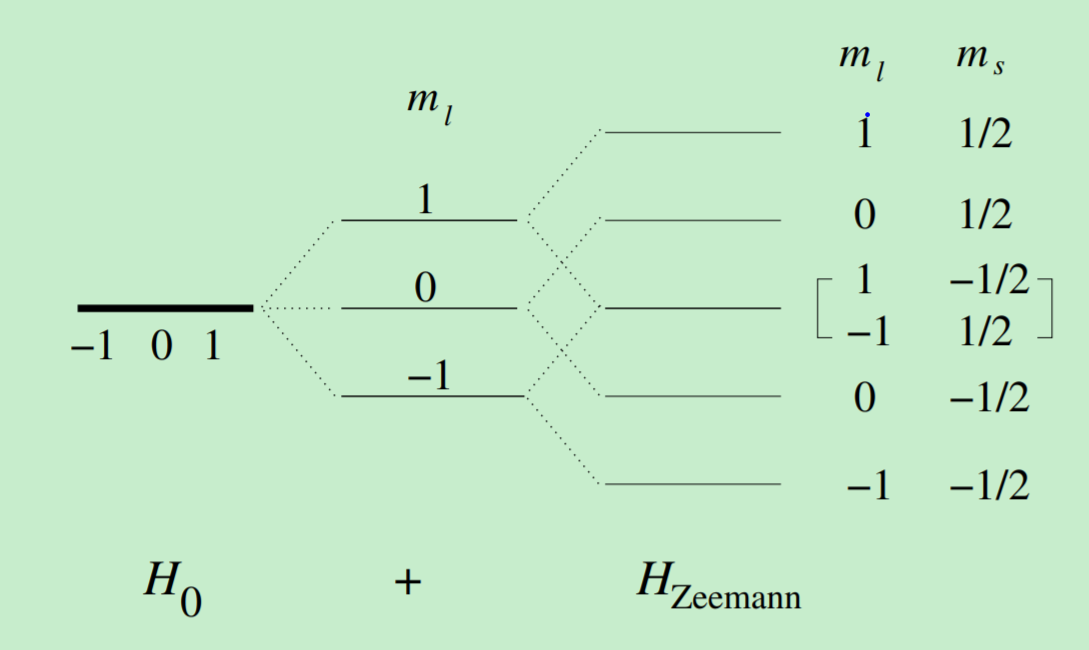
\includegraphics[scale=1]{11_12.PNG}
        \captionsetup{font={Large}}
        \caption{Zeeman splits in a hydrogen atom 6 = 2 × 3 times (spin × orbit) $ p $ state. The orbital moment produces a triplet state with two degenerate states (rotations). The landing factor of electron spin $ g \approx 2 $ only compensates for half of the spin moment, so the orbit and spin lead to the same energy split and produce a quintet state with a degenerate central state.}
\end{figure}
With
%公式 109
\begin{equation}
    \left\langle\frac{1}{r^{3}}\right\rangle_{n l}=\frac{1}{a_{B}^{3}} \frac{1}{n^{3}} \frac{1}{l\left(l+\frac{1}{2}\right)(l+1)}
    \end{equation}
and
%公式 110
\begin{equation}
\begin{aligned} \frac{e^{2} \hbar^{2}}{m^{2} c^{2}} &=\frac{e^{4}}{\hbar^{2} c^{2}} \frac{\hbar^{4}}{e^{2} m^{2}}=\alpha^{2} e^{2} a_{B}^{2} \\ \frac{e^{4} m}{2 \hbar^{2}} &=\frac{e^{2}}{2 a_{B}}=E_{R}=13.6 \mathrm{eV} \end{aligned}
\end{equation}
the splitting results
%公式 111
\begin{equation}
\Delta E_{\mathrm{SO}}=\frac{\alpha^{2} E_{R}}{2 n^{3}} \frac{1}{l\left(1+\frac{1}{2}\right)(l+1)}\left(\begin{array}{c}{l} \\ {-(l+1)}\end{array}\right)=\frac{\alpha^{2}\left|E_{n}\right|}{2 n\left(l+\frac{1}{2}\right)}\left(\begin{array}{c}{1 /(l+1)} \\ {-1 / l}\end{array}\right)
\end{equation}
The comparison of the order of magn
%公式 112
\begin{equation}
    \frac{\Delta E_{\mathrm{SO}}}{\Delta E_{\mathrm{Z}}} \sim \frac{\alpha^{2} E_{R}}{\mu_{B} \mathrm{H}_{z}}=\frac{1}{137^{2}} \frac{13.6}{5.8 \cdot 10^{-9}} \frac{1}{\mathrm{H}_{z}[\mathrm{G}]}=1.25 \cdot 10^{5} / \mathrm{H}_{z}[G]
    \end{equation}
this means that $\Delta E_{\mathrm{SO}}>\Delta E_{\mathrm{Z}}$ for $\mathrm{H}_{z}<10^{5}$ Gauss. In Chapter 14 we will discuss the additional Zeeman splitting in small fields.\par
An electron ($e> 0$) with spin which (slow, non-relativistic, we are not looking at the hydrogen atom here) moves in the electromagnetic fields $\vec{A}$ and $\varphi$ is described by the Pauli equation,
%公式 113
\begin{equation}
\begin{aligned} 
i \hbar \partial_{t}\left(\begin{array}{c}{\Psi_{\uparrow}(\vec{r}, t)} \\ {\Psi_{\downarrow}(\vec{r}, t)}\end{array}\right)=\left[\frac{1}{2 m}\left(\frac{\hbar}{i} \vec{\nabla}+\frac{e}{c} \vec{A}(\vec{r}, t)\right)^{2}\right.\cdot\mathbb{1} \\ \qquad\qquad\qquad\left.+\frac{g \mu_{B}}{2} \vec{\sigma} \cdot \vec{H}(\vec{r}, t)-e \varphi(\vec{r}, t) \mathbb{1}\right]\left(\begin{array}{l}{\Psi_{\uparrow}(\vec{r}, t)} \\ {\Psi_{\downarrow}(\vec{r}, t)}\end{array}\right) \end{aligned}
\end{equation}